% This is samplepaper.tex, a sample chapter demonstrating the
% LLNCS macro package for Springer Computer Science proceedings;
% Version 2.20 of 2017/10/04
%
\documentclass[runningheads]{llncs}
%
\usepackage{graphicx}
\usepackage{tikz}
\usepackage{subcaption}
\captionsetup{compatibility=false}
\newcommand*\rot{\rotatebox{90}}
\usepackage{amssymb}
\usetikzlibrary{positioning}

\usetikzlibrary{arrows}

\usepackage{amsmath}
\usepackage{booktabs}
\usepackage[ruled,noend,vlined,linesnumbered]{algorithm2e}
\usepackage{footmisc}

% Used for displaying a sample figure. If possible, figure files should
% be included in EPS format.
%
% If you use the hyperref package, please uncomment the following line
% to display URLs in blue roman font according to Springer's eBook style:
% \renewcommand\UrlFont{\color{blue}\rmfamily}
\usepackage{color}


\usepackage{color}
% latex if conditions
\newif\ifdraft\drafttrue
\newif\ifreviewChanges\reviewChangestrue
\newif\ifinlineref\inlinereffalse
\newif\iffinal\finalfalse
\newif\ifextended\extendedfalse
\newif\ifdotikz\dotikzfalse
\newif\ifmakeallproofsinline\makeallproofsinlinefalse


%set flags
\draftfalse
\finalfalse
\reviewChangesfalse


\ifdraft
%\ifreviewChanges
%\newcommand{\comment}[1]{{\textcolor{blue}{*** #1 ***}}}
\newcommand{\thi}[1]{{\textcolor{red}{ *TH: #1 * }}}
\newcommand{\gad}[1]{{\textcolor{blue}{ *G: #1 * }}}
\newcommand{\ds}[1]{{\textbf{\textcolor{olivegreen}{ *D: #1 * }}}}
\newcommand{\evgeny}[1]{\textbf{\color{red}*Evgeny: #1 *}}


\else
\newcommand{\thi}[1]{}
\newcommand{\gad}[1]{}
\newcommand{\ds}[1]{}
\newcommand{\evgeny}[1]{}


\fi

%Defined by Gad
\ifreviewChanges
\newcommand{\dl}[1]{{\color{darkred} #1}}
\newcommand{\add}[1]{{\color{olivegreen} #1}}
\else
\newcommand{\dl}[1]{}
\newcommand{\add}[1]{#1}
\fi



\newcommand{\missing}[1]{{\color{red}\textit{#1?}}}
%!TEX root = main.tex
\usepackage{color}



\definecolor{darkred}{RGB}{139, 0, 0}
\definecolor{olivegreen}{RGB}{0, 110, 0}
\newcommand{\calcic}{\calc^{\subseteq}}

\newcommand{\ICs}{\mathcal{C}}
\newcommand{\Cl}{\mathit{Cl}}

%\newtheorem{dtheorem}[theorem]{Theorem}
\newcommand{\NP}{\mathsf{NP}}
\newcommand{\NLOG}{\mathsf{NLogSpace}}
\newcommand{\LOG}{\mathsf{LogSpace}}
\newcommand{\ACzero}{\mathsf{AC}^0}

\newcommand{\leanparagraph}[1]{\smallskip\noindent\textbf{#1}. }

\newcommand{\nop}[1]{}

\newcommand{\calc}{\mathcal{K}_{\mathit{taut}}}

\newcommand{\dlf}[1]{\mathcal{#1}}
\def\rel#1{\mbox{\small\textsc{#1}}}
\def\conc#1{\mbox{\textsf{#1}}}
\def\inst#1{\mbox{\small{\texttt{#1}}}}
\def\axiom#1{\mbox{\textit{#1}}}
\def\var#1{\mbox{\textsl{#1}}}
\def\code#1{\mbox{\small{\texttt{#1}}}}
\def\lex#1{\mbox{{\small``\textsf{#1}''}}}

\makeatletter
\providecommand{\leftsquigarrow}{%
  \mathrel{\mathpalette\reflect@squig\relax}%
}
\newcommand{\reflect@squig}[2]{%
  \reflectbox{$\m@th#1\rightsquigarrow$}%
}
\makeatother

\def\impliedBy{\leftarrow}
\def\la{\leftarrow}
\def\slot{\rightarrow\hspace{-1.3ex}\rightarrow}
\def\tslot{\Rightarrow\hspace{-1.3ex}\Rightarrow}

\newcommand{\dlpluslog}{\ensuremath{\mathcal{DL}\text{+}\mathit{log}}}


\newcommand{\redx}{\ensuremath{\lp^M_x}\xspace}
\newcommand{\redinter}{\ensuremath{\lp^M_\inter}\xspace}

\newcommand{\flpfred}[2]{\ensuremath{{#1^{#2}_{\mathit{f}}}}\xspace}
\newcommand{\flpnred}[2]{\ensuremath{{#1^{#2}_{\mathit{t}}}}\xspace}
\newcommand{\flpcred}[2]{\ensuremath{{#1^{#2}_{\mathit{c}}}}\xspace}
\newcommand{\flpredas}[2]{\ensuremath{{#1^{#2}_{\mathit{FLP}}}}\xspace}
\newcommand{\flpreddllp}[3]{\ensuremath{{#1^{#2,#3}_{\mathit{FLP}}}}\xspace}
\newcommand{\glredas}[2]{\ensuremath{{#1^{#2}_{\mathit{GL}}}}\xspace}
\newcommand{\dlpred}[2]{\ensuremath{{#1^{#2}_{\mathit{d}}}}\xspace}
\newcommand{\strred}[2]{\ensuremath{{#1^{#2}_{\mathit{s}}}}\xspace}
%\newcommand{\conf}[1]{\ensuremath{{\mathit{conf}(#1)}}\xspace}

\newcommand{\atom}[2]{\ensuremath{\mathit{#1}(#2)}\xspace}
\newcommand{\ew}[2]{\ensuremath{\mathbf{EW}(\mathit{#1},{#2})}\xspace}
\newcommand{\dlpropatom}[2]{\ensuremath{{
\mathrm{DL}[#1;\,#2]
}}\xspace}

\newcommand{\dlatom}[3]{\ensuremath{{
\dlpropatom{#1}{#2}(#3)
}}\xspace}
%\newcommand{\h}[1]{\ensuremath{\mi{Head()}}}
\newcommand{\ddlatom}[5]{\ensuremath{
\begin{array}{@{}r@{}l@{}}
\mathrm{DL}[#1,& #2 \\
               & #3;\, #4](#5)
\end{array}
}\xspace}

\newcommand{\redfot}{\ensuremath{\lp^M_\fot}\xspace}

\newcommand{\mop}{\ensuremath{\mathsf{L}}\xspace}
\newcommand{\mopb}{\ensuremath{\mathsf{B}}\xspace}
\newcommand{\mopm}{\ensuremath{\mathsf{M}}\xspace}
\newcommand{\mopo}{\ensuremath{\mathsf{O}}\xspace}

\newcommand{\limpl}{\ensuremath{\supset}}
\newcommand{\dnot}{\ensuremath{not\text{ }}}
\newcommand{\snot}{\ensuremath{\sim}\xspace}

\newcommand{\domain}{\ensuremath{U}\xspace}
\newcommand{\sinter}{\ensuremath{\mathbf{I}}\xspace}
\newcommand{\minter}{\ensuremath{\langle \inter, \sinter \rangle}\xspace}
\newcommand{\hinter}{\ensuremath{I}\xspace}
\newcommand{\inter}{\ensuremath{\mathcal{I}}\xspace}
\newcommand{\interfunsym}{\ensuremath{\inter}\xspace}
\newcommand{\interfun}{\ensuremath{\cdot^\interfunsym}\xspace}
\newcommand{\interdef}{\ensuremath{\inter = \langle \domain, \interfun
  \rangle}\xspace}

\newcommand{\logic}{\ensuremath{\mathscr{L}}\xspace}
\newcommand{\lang}{\ensuremath{\mathcal{L}}\xspace}
\newcommand{\flang}{\ensuremath{\mathcal{L}}\xspace}

\newcommand{\fsymb}{\ensuremath{\mathcal{F}}\xspace}
\newcommand{\psymb}{\ensuremath{\mathcal{P}}\xspace}
\newcommand{\psymbc}{\ensuremath{\mathcal{P}_\mathit{c}}\xspace}
\newcommand{\psymbr}{\ensuremath{\mathcal{P}_\mathit{r}}\xspace}
\newcommand{\psymbdl}{\ensuremath{\mathcal{P}_\mathit{o}}\xspace}
\newcommand{\psymblp}{\ensuremath{\mathcal{P}_\mathit{p}}\xspace}
\newcommand{\psymblpi}{\psymblp^{({-})}}
\newcommand{\csymb}{\ensuremath{\mathcal{C}}\xspace}
\newcommand{\vsymb}{\ensuremath{\mathcal{V}}\xspace}

\newcommand{\signature}{\ensuremath{\Sigma}\xspace}
\newcommand{\signaturelp}{\ensuremath{\Sigma_\mathit{p}}\xspace}
\newcommand{\signaturedl}{\ensuremath{\Sigma_\mathit{o}}\xspace}


\newcommand{\dlpsigdef}{\ensuremath{\signature=\langle \fsymb,\psymbdl,\psymblp\rangle}\xspace}
\newcommand{\sigdefdl}{\ensuremath{\signaturedl=\langle \fsymb,\psymbdl\rangle}\xspace}
\newcommand{\sigdeflp}{\ensuremath{\signaturelp=\langle \fsymb,\psymblp\rangle}\xspace}


\newcommand{\hu}{\ensuremath{\mathrm{HU}}\xspace}
\newcommand{\hb}{\ensuremath{\mathrm{HB}}\xspace}

\newcommand{\head}[1]{\ensuremath{H(#1)}\xspace}
\newcommand{\body}[1]{\ensuremath{B(#1)}\xspace}
\newcommand{\pbody}[1]{\ensuremath{B(#1)^+}\xspace}
\newcommand{\nbody}[1]{\ensuremath{B(#1)^-}\xspace}

\newcommand{\HBi}[3]{\ensuremath{\hb_{#1,#2}(#3)}\xspace}
\newcommand{\HBis}[3]{\ensuremath{\hb_{#1,#2}^*(#3)}\xspace}
\newcommand{\HB}[1]{\ensuremath{\hb(#1)}\xspace}
\newcommand{\HU}[1]{\ensuremath{\hu(#1)}\xspace}

\newcommand{\DLA}[1]{\ensuremath{\mathrm{D({#1})}}\xspace}
\newcommand{\DLAq}{\ensuremath{\mathrm{DL}^{?}}\xspace}
\newcommand{\DLAp}{\ensuremath{\mathrm{DL}^{+}}\xspace}

\newcommand{\DLApm}{\ensuremath{\mathrm{DL}_{m}^{+}}\xspace}
\newcommand{\DLApa}{\ensuremath{\mathrm{DL}_{a}^{+}}\xspace}
\newcommand{\DLAqm}{\ensuremath{\mathrm{DL}_{m}^{?}}\xspace}
\newcommand{\DLAqa}{\ensuremath{\mathrm{DL}_{a}^{?}}\xspace}

\newcommand{\DLAm}{\ensuremath{\mathrm{DL}}\xspace}


\newcommand{\hm}{\ensuremath{HM}\xspace}

\newcommand{\gr}[1]{\ensuremath{gr(#1)}\xspace}
\newcommand{\grset}[2]{\ensuremath{gr_{#2}(#1)}\xspace}
\newcommand{\gro}[1]{\ensuremath{gr_o(#1)}\xspace}

\newcommand{\AS}[1]{\ensuremath{\mathrm{AS}(#1)}\xspace}
\newcommand{\cAS}[1]{\ensuremath{\mathrm{AS^c}(#1)}\xspace}
\newcommand{\fAS}[1]{\ensuremath{\mathrm{AS^f}(#1)}\xspace}
\newcommand{\nAS}[1]{\ensuremath{\mathrm{AS^t}(#1)}\xspace}

\newcommand{\lp}{\ensuremath{\Pi}\xspace}
\newcommand{\DL}{\fot}
\newcommand{\fot}{\ensuremath{\cO}\xspace}

\newcommand{\modl}{\ensuremath{\lang_{\mop}}\xspace}
\newcommand{\fmodl}{\ensuremath{\flang_{\mop}}\xspace}
\newcommand{\fmodlcomb}{\ensuremath{\flang_{\mop}^{\flang \cup \lp}\xspace}}
\newcommand{\fmodlnoq}{\ensuremath{\fmodl'}\xspace}

\newcommand{\varsub}{\ensuremath{\beta}\xspace}
\newcommand{\varass}{\ensuremath{B}\xspace}

\newcommand{\shoiqd}{\ensuremath{\mathcal{SHOIQ}(\mathbf{D})}\xspace}
\newcommand{\dlr}{\ensuremath{\mathcal{DLR}}\xspace}
\newcommand{\dlrom}{\ensuremath{\mathcal{DLRO}^{-\{\leq\}}}}
\newcommand{\dlro}{\ensuremath{\mathcal{DLRO}}}
\newcommand{\shoind}{\ensuremath{\mathcal{SHOIN}(\mathbf{D})}\xspace}
\newcommand{\shoiq}{\ensuremath{\mathcal{SHOIQ}}\xspace}
\newcommand{\shoq}{\ensuremath{\mathcal{SHOQ}}\xspace}
\newcommand{\sroiq}{\ensuremath{\mathcal{SROIQ}}\xspace}
\newcommand{\shif}{\ensuremath{\mathcal{SHIF}}\xspace}
\newcommand{\shifd}{\ensuremath{\mathcal{SHIF}(\mathbf{D})}\xspace}
\newcommand{\shiq}{\ensuremath{\mathcal{SHIQ}}\xspace}
\newcommand{\shiqd}{\ensuremath{\mathcal{SHIQ}(\mathbf{D})}\xspace}
\newcommand{\shoin}{\ensuremath{\mathcal{SHOIN}}\xspace}
\newcommand{\alc}{\ensuremath{\mathcal{ALC}}\xspace}
\newcommand{\alchiq}{\ensuremath{\mathcal{ALCHIQ}}\xspace}
\newcommand{\alcnr}{\ensuremath{\mathcal{ALCNR}}\xspace}
\newcommand{\elpp}{\ensuremath{\mathcal{EL}^{++}}\xspace}
\newcommand{\dllite}{\ensuremath{\mathit{DL\text{-}Lite}}\xspace}


\newcommand{\datalog}{\textsc{Datalog}\xspace}
\newcommand{\datalogv}{$\mbox{\textsc{Datalog}}^{\lor}$\xspace}
\newcommand{\datalogn}{$\mbox{\textsc{Datalog}}^{\neg}$\xspace}
\newcommand{\datalogvn}{$\mbox{\textsc{Datalog}}^{\lor,\neg}$\xspace}

\newcommand{\wrt}{w.r.t.\xspace}
\newcommand{\ie}{\emph{i.e.},\xspace}
\newcommand{\eg}{\emph{e.g.},\xspace}
\newcommand{\vs}{\emph{vs}.\xspace}
\newcommand{\etc}{\emph{etc}\onedot}

\newcommand{\dllog}{$\dlf{DL}$\mbox{+}\textsc{log}\xspace}
\newcommand{\comblog}[1]{$\dlf{#1}$\mbox{+}\textsc{log}\xspace}



\newcommand{\dlvhex}{DLVHEX\xspace}

%% COMPLEXITY CLASSES



\newcommand{\logspace}{\textsc{LogSpace}\xspace}

\newcommand{\nlogspace}{\textsc{NLogSpace}\xspace}

\newcommand{\ptime}{\textsc{PTime}\xspace}

\newcommand{\p}{\textsc{P}\xspace}
\newcommand{\pc}{\textsc{P}\complete\xspace}

\newcommand{\ph}{\textsc{PH}\xspace}

\newcommand{\np}{\textsc{NP}\xspace}
\newcommand{\complete}{\text{-complete}}
\newcommand{\completeness}{\text{-completeness}}
\newcommand{\npc}{\textsc{NP}\complete\xspace}

\newcommand{\conp}{\textsc{co-NP}\xspace}
\newcommand{\conpc}{\textsc{co-NP}\complete\xspace}

\newcommand{\pip}[1]{\ensuremath{\Pi^P_{#1}}\xspace}
\newcommand{\sigmap}[1]{\ensuremath{\Sigma^P_{#1}}\xspace}
\newcommand{\deltap}[1]{\ensuremath{\Delta^P_{#1}}\xspace}

\newcommand{\transflpsem}[1]{\ensuremath{\rho({#1})}\xspace}
\newcommand{\transposdlsimnormal}[1]{\ensuremath{\nu({#1})}\xspace}


\newcommand{\pspace}{\textsc{PSpace}\xspace}

\newcommand{\psp}{\pspace}

\newcommand{\exptime}{\textsc{ExpTime}\xspace}
\newcommand{\exptimec}{\textsc{ExpTime}\complete\xspace}
\newcommand{\exptimecs}{\textsc{ExpTime}\completeness\xspace}

%\newcommand{\C}{\textsc{C}\xspace}
\newcommand{\nexptime}{\textsc{NExpTime}\xspace}
\newcommand{\nexptimec}{\textsc{NExpTime}\complete\xspace}
\newcommand{\nexptimecs}{\textsc{NExpTime}\completeness\xspace}
\newcommand{\nexp}{\textsc{NExp}\xspace}
\newcommand{\nexpc}{\textsc{NExp}\complete\xspace}

\newcommand{\conexptime}{\textsc{co-NExpTime}\xspace}
\newcommand{\conexp}{\textsc{co-NExp}\xspace}
\newcommand{\conexpc}{\textsc{co-NExp}\complete\xspace}

\newcommand{\exptimen}[1]{\textsc{{#1}ExpTime}\xspace}

\newcommand{\nnexptime}[1]{\textsc{{#1}NExpTime}\xspace}


\newcommand{\nconexptime}[1]{\textsc{co-{#1}NExpTime}\xspace}

\newcommand{\nexptimeNP}{\ensuremath{\textsc{NExpTime}^\textsc{NP}}\xspace}



\newcommand{\ckb}{\ensuremath{\mathcal{KB}}\xspace}



\newcommand{\ckbdef}{\ensuremath{\mathcal{KB} = \langle \fot, \lp
    \rangle}\xspace}

%\newcommand{\citeN}[1]{\protect\citeauthor{#1}~\shortcite{#1}\protect}


\newcommand{\dlextension}[2]{\ensuremath{\tau^{#1}(#2)}}

% queries
% certain answers
\newcommand{\cansw}[2]{\ensuremath{\mathit{cansw}(#1,#2)}}
% skeptical answers
\newcommand{\pansw}[2]{\ensuremath{\mathit{pansw}(#1,#2)}}

%\newcommand{\st}{\ensuremath{\,.\,}}
\newcommand{\names}{\ensuremath{\mathcal{N}}\xspace}

% DL-program
%\newcommand{\dlpdef}{\ensuremath{\dlp=(\DL,\lp)}\xspace}
\newcommand{\dlpdef}{\ensuremath{P=(\DL,\lp)}\xspace}
\newcommand{\dlp}{\ensuremath{\mathcal{KB}}\xspace}

\newcommand{\dlpi}[2]{\ensuremath{\mathcal{KB}_{#1,#2}}\xspace}
\newcommand{\dlpis}[2]{\ensuremath{\mathcal{KB}_{#1,#2}^*}\xspace}

\newcommand{\lpis}[2]{\ensuremath{\lp_{#1,#2}^*}\xspace}
\newcommand{\tuple}[1]{\langle#1\rangle}
\newcommand{\cA}{\mathcal{A}}
\newcommand{\cC}{\mathcal{C}}
\newcommand{\cG}{\mathcal{G}}
\newcommand{\cO}{\mathcal{O}}
\newcommand{\cP}{\mathcal{P}}
\newcommand{\cT}{\mathcal{T}}
\newcommand{\cS}{\mathcal{S}}
\newcommand{\cL}{\mathcal{L}}
\newcommand{\cN}{\mathcal{N}}
\newcommand{\cH}{\mathcal{H}}
\newcommand{\cU}{\mathcal{U}}
\newcommand{\bR}{\mathbf{R}}
\newcommand{\bC}{\mathbf{C}}
\newcommand{\bI}{\mathbf{I}}
\newcommand{\bS}{\mathbf{S}}
\newcommand{\bP}{\mathbf{P}}
\newcommand{\cR}{\mathcal{R}}
\newcommand{\myequation}[4]{%
\newcommand{\h}
\vspace*{#1\baselineskip}

\begin{equation}
\label{#2}
#3
\end{equation}

\vspace*{#4\baselineskip}
}


\newcommand{\FLP}{\ensuremath{\mathit{flp}}\xspace}

\newcommand{\mi}[1]{\mathit{#1}}
\newcommand{\Supp}{\mi{Supp}}

\newcommand{\NewRAnsSet}{\ensuremath{\mathit{SupRAnsSet}}}


\newcounter{myenumctr}
\newenvironment{myenumerate}{\begin{list}{(\arabic{myenumctr})}{\usecounter{myenumctr}
\topsep=0pt
\setlength{\leftmargin}{0.5\labelwidth}
\setlength{\itemindent}{1.5\labelwidth}
\setlength{\itemsep}{0cm}}}
{\end{list}}



% definition of uminus operator sign

\def\uminus{\setbox0=\hbox{$\cup$}\rlap{\hbox
    to\wd0{\hss\raise0.3ex\hbox{$\scriptscriptstyle{-}$}\hss}}\box0}

\def\uminusstar{\setbox0=\hbox{$\cup$}\rlap{\hbox
    to\wd0{\hss\raise0.3ex\hbox{$\scriptscriptstyle{-^\star}$}\hss}}\box0}


% definition of alternative uplus operator sign

\def\myuplus{\setbox0=\hbox{$\cup$}\rlap{\hbox
    to\wd0{\hss\raise0.4ex\hbox{$\scriptscriptstyle{+}$}\hss}}\box0}


% definition of capminus operator sign

\def\cminus{\setbox0=\hbox{$\cap$}\rlap{\hbox
    to\wd0{\hss\raise0.3ex\hbox{$\scriptscriptstyle{-}$}\hss}}\box0}


\def\cminusstar{\setbox0=\hbox{$\cap$}\rlap{\hbox
    to\wd0{\hss\raise0.3ex\hbox{$\scriptscriptstyle{-}$}\hss}}\box0^\star}

\newcommand{\lpor}{\mid}

\newcommand{\naf}[1]{\ensuremath{\mathit{not}~ #1}}

\newcommand{\uplusc}{\ensuremath{\uplus_c}}
\newcommand{\uminusc}{\ensuremath{\uminus_c}}
\newcommand{\cminusc}{\ensuremath{\cminus_c}}

\newcommand{\uplusi}{\ensuremath{\uplus_i}}
\newcommand{\uminusi}{\ensuremath{\uminus_i}}
\newcommand{\cminusi}{\ensuremath{\cminus_i}}

\newcommand{\upluso}{\ensuremath{\uplus_\mathrm{opt}}}
\newcommand{\uminuso}{\ensuremath{\uminus_\mathrm{opt}}}
\newcommand{\cminuso}{\ensuremath{\cminus_\mathrm{opt}}}
% A single rule outside a program.
\newcommand{\prule}[2]{\ensuremath{\mathit{#1}\gets\mathit{#2}}}

% stable model of a Combined KB:
%\newcommand{\smodels}{\ensuremath{\models_s}}

% for logic programs
\newenvironment{program}{\[\begin{array}{rll}}{\end{array}\]}
\newcommand{\tsrule}[2]{\ensuremath{\mathit{#1} &\gets& \mathit{#2}\\}}


\newcommand{\mknflang}{\ensuremath{\lang_{\mathit{MKNF}}}\xspace}
\newcommand{\mknfmodels}{\ensuremath{\models^{\mopk,\mopnot}}\xspace}
\newcommand{\ssmodels}{\ensuremath{\models_{S5}}\xspace}

\newcommand{\amodels}{\ensuremath{\models_{\mathit{a}}}\xspace}
\newcommand{\cmodels}{\ensuremath{\models_{\mathit{c}}}\xspace}
\newcommand{\fmodels}{\ensuremath{\models_{\mathit{f}}}\xspace}
\newcommand{\nmodels}{\ensuremath{\models_{\mathit{t}}}\xspace}


\newcommand{\mknfinter}{\ensuremath{M}\xspace}
\newcommand{\mknfstructure}{\ensuremath{(\inter, \mknfinter, N)}\xspace}


\newcommand{\mopk}{\ensuremath{\mathsf{K}}\xspace}
\newcommand{\mopnot}{\ensuremath{\mathsf{not}}\,}

% more compact itemize environments
\newenvironment{myitemize}
   {\begin{itemize}\setlength{\itemsep}{-0.08cm}}{\end{itemize}}


\newcommand{\be}{\begin{enumerate}}
\newcommand{\ee}{\end{enumerate}}

\newcommand{\shoinSWRL}{\shoin-SWRL\xspace}

\newcommand{\smallfol}{{\text{\footnotesize{+FOL}}}}
\newcommand{\smalldl}{{\text{\footnotesize{+DL}}}}
\newcommand{\folflogic}{$\text{F}^{\smallfol}\text{-Logic}$\xspace}
\newcommand{\dlflogic}{$\text{F}^{\smalldl}\text{-Logic}$\xspace}
\newcommand{\folfmodels}[1]{\ensuremath{{\ \models_{\mathsf{f},#1}\ }}\xspace}
\newcommand{\nfolfmodels}[1]{\ensuremath{{\ \nmodels_{\mathsf{f},#1}\ }}\xspace}

%\newcommand{\DLmodels}{\ensuremath{{\ \models_\DL\ }}\xspace}
\newcommand{\cdlmodels}{\ensuremath{{\ \models_{\DL,c}\ }}\xspace}

% combined signature
\newcommand{\csig}{\ensuremath{\langle \signature_\Phi, \signature_P \rangle}\xspace}

\newcommand{\attr}[1]{\ensuremath{\twoheadrightarrow\!\!#1}\xspace}
\newcommand{\type}[1]{\ensuremath{:\!\!#1}\xspace}
\def\bD{\mathbf{D}}
%\newcommand{\cE}{{\mathbf E}}
%\newcommand{\cR}{{\mathbf R}}
\newcommand{\cE}{\mathcal{E}}
\newcommand{\cV}{{\mathbf V}}



\def\DLB{{\it L}}
\newcommand{\bt}{\begin{tabular}}
\def\cI{{\cal I}}


\newcommand{\et}{\end{tabular}}
\newcommand{\bs}{\begin{theorem}}
\newcommand{\es}{\end{theorem}}
\newcommand{\bsw}[1]{\begin{theorem}[#1]}
\newcommand{\esw}{\end{theorem}}
\newcommand{\bc}{\begin{corollary}}
\newcommand{\ec}{\end{corollary}}
\newcommand{\bcw}[1]{\begin{corollary}[#1]}
\newcommand{\ecw}{\end{corollary}}
\newcommand{\ble}{\begin{lemma}}
\newcommand{\ele}{\end{lemma}}
\newcommand{\blew}[1]{\begin{lemma}[#1]}
\newcommand{\elew}{\end{lemma}}
\newcommand{\bp}{\begin{proposition}}
\newcommand{\ep}{\end{proposition}}
\newcommand{\bd}{\begin{definition}\rm}
\newcommand{\ed}{\end{definition}}
\newcommand{\bdw}[1]{\begin{definition}[\textit{#1}]\rm}
\newcommand{\edw}{\end{definition}}
\newcommand{\ba}{\begin{algorithm}\rm}
\newcommand{\ea}{\end{algorithm}}
\newcommand{\baw}[1]{\begin{algorithm}[#1]\rm}
\newcommand{\eaw}{\end{algorithm}}
\newcommand{\bbs}{\begin{example}\rm}
\newcommand{\ebs}{\end{example}}
\newcommand{\bbsw}[1]{\begin{example}[#1]\rm}
\newcommand{\ebsw}{\end{example}}
\newcommand{\bb}{\begin{remark}\rm}
\newcommand{\eb}{\end{remark}}
\newcommand{\beq}{\begin{eqnarray*}}
\newcommand{\eeq}{\end{eqnarray*}}
\newcommand{\baq}{\begin{array}}
\newcommand{\eaq}{\end{array}}


\newcommand{\mids}{\,{\mid}\,}
\newcommand{\ins}{\,{\in}\,}
\newcommand{\gts}{\,{>}\,}
\newcommand{\ges}{\,{\ge}\,}
\newcommand{\les}{\,{\le}\,}
\newcommand{\lts}{\,{<}\,}
\newcommand{\eqs}{\,{=}\,}
\newcommand{\eq}{\ensuremath{\eqs\!}}
\newcommand{\diff}{\ensuremath{\neqs\!}}
\newcommand{\neqs}{\,{\neq}\,}
\newcommand{\modelss}{\,{\models}\,}
\newcommand{\notmodelss}{\,{\not\models}\,}
\newcommand{\cups}{\,{\cup}\,}
%\newcommand{\caps}{\,{\cap}\,}
\newcommand{\subseteqs}{\,{\subseteq}\,}
\newcommand{\sqsubseteqs}{\,{\sqsubseteq}\,}





\begin{document}
%
\title{Rule Induction and Reasoning over\\ Knowledge Graphs}
%
%\titlerunning{Abbreviated paper title}
% If the paper title is too long for the running head, you can set
% an abbreviated paper title here
%
\author{First Author\inst{1} \and
Second Author\inst{1} \and
Third Author\inst{1}}


%
\authorrunning{F. Author et al.}
% First names are abbreviated in the running head.
% If there are more than two authors, 'et al.' is used.
%
\institute{Max Planck Institute for Informatics,\\ Saarland Informatics Campus, Germany\\
\email{lncs@springer.com}\\
%\url{http://www.springer.com/gp/computer-science/lncs} \and
%ABC Institute, Rupert-Karls-University Heidelberg, Heidelberg, Germany\\
%\email{\{abc,lncs\}@uni-heidelberg.de}
}
%
\maketitle              % typeset the header of the contribution
%
\begin{abstract}
Advances in information extraction have enabled the automatic
construction of large knowledge graphs (KGs) like DBpedia, Freebase, YAGO
and Wikidata. Learning rules from KGs is a crucial task for KG completion,
cleaning and curation. This tutorial presents state-of-the-art rule
induction methods, recent advances, research opportunities as well as open
challenges along this avenue. We put a particular emphasis on the problems
of learning exception-enriched rules from highly biased and incomplete
data. Finally, we discuss possible extensions of classical rule induction
techniques to account for unstructured resources (e.g., text) along with
the structured ones.
%\keywords{First keyword  \and Second keyword \and Another keyword.}
\end{abstract}



\section{Introduction}
%(2 pages)}
\label{sec:intro}

\leanparagraph{Motivation}
Recent advances in information extraction have led to
huge graph-structured knowledge bases (KBs) also known as knowledge graphs (KGs) such as NELL \cite{nell}, DBpedia \cite{dbpedia}, YAGO \cite{yago} and Wikidata \cite{wikidata}. These KGs contain millions or billions of relational facts in the form of subject-predicate-object (SPO) triples, e.g., $\tuple{\mi{clara\;isMarriedTo\;dave}}$ or $\tuple{\mi{dave\;isA\;researcher}}$. Such triples can be straightforwardly represented by means of positive unary and binary first-order logic facts, e.g. $\mi{marriedTo(clara,dave)}$ and $\mi{researcher(dave)}$.

An important task over KGs is rule learning, which is relevant for a variety of applications ranging from knowledge graph curation (completion, error detection) \cite{DBLP:journals/semweb/Paulheim17} to data mining and semantic culturonomics. Rules over KGs are of the form $\mi{head \leftarrow body}$, where $\mi{head}$ is a binary atom and $\mi{body}$ is a conjunction of, possibly negated, binary and unary atoms. 
Traditionally, rule induction has been studied in the context of relational data mining in databases (see e.g., \cite{DBLP:books/daglib/0021868} for overview), and has recently been adapted to KGs (e.g., \cite{amie,op,rdf2rules}). The methods from this area can be used to identify prominent patterns from KGs, such as \emph{``Married people live in the same
place''}, and cast them in the form of Horn rules, such as:
$\mi{r_1:\;}\mi{livesIn(Y,Z)}\leftarrow \mi{isMarriedTo(X,Y),livesIn(X,Z)}$. 

For the KG curation, this has two-fold benefits. First, since KGs operate under the Open World
Assumption (OWA) (i.e., absent facts are treated as unknown rather than false),
the rules can be used to derive additional facts such as missing living places. % For example, applying the rule
% $\mi{r_1}$ mined from the graph in Figure~\ref{rdf}, the missing living places of Dave and Lucy can be deduced based on the data about their spouses.
Second, rules can be used to eliminate erroneous facts in KGs. For example, assuming that $\mi{livesIn}$ is a functional relation, % Amsterdam as a 
a living place of a person could be questioned if it differs from the spouse's.

When rules are automatically learned, statistical measures like support, confidence and their variations are used to asssess the rules' quality. Most notably, the confidence of a rule is the fraction of facts predicted by the rule that are indeed in the KG. However, this is a meaningful measure for rule quality only when the KG is reasonably complete. For rules learned from incomplete KGs, confidence and other measures may be misleading, as they do not reflect the patterns in the missing facts. This might lead to the extraction of erroneous rules from incomplete and biased KGs. For example, a KG that knows a lot of information about families of popular scientists but lacks data in other domains, would yield a heavily biased rule $\mi{r_1':hasChild(X,Y)\leftarrow worksAt(X,Z), educated(Y,Z)}$, stating that workers of certain institutions often have children among the people educated there, as this is frequently the case for scientific families. To address this issue, several rule measures that are specifically tailored towards incomplete KGs have been proposed \cite{amie,DBLP:conf/www/ZupancD18} (see \cite{metrics-summary,Azevedo2007} for an overview of other measures). Along with KGs themselves, additional meta data about the concrete numbers of facts of certain types that hold in the real world (e.g., \emph{``Einstein has 3 children''}) could be exploited in rule learning to better assess the quality of the induced rules \cite{carl}. 

\begin{figure}[t]
\centering
\begin{subfigure}[b]{0.75\textwidth}
    \centering
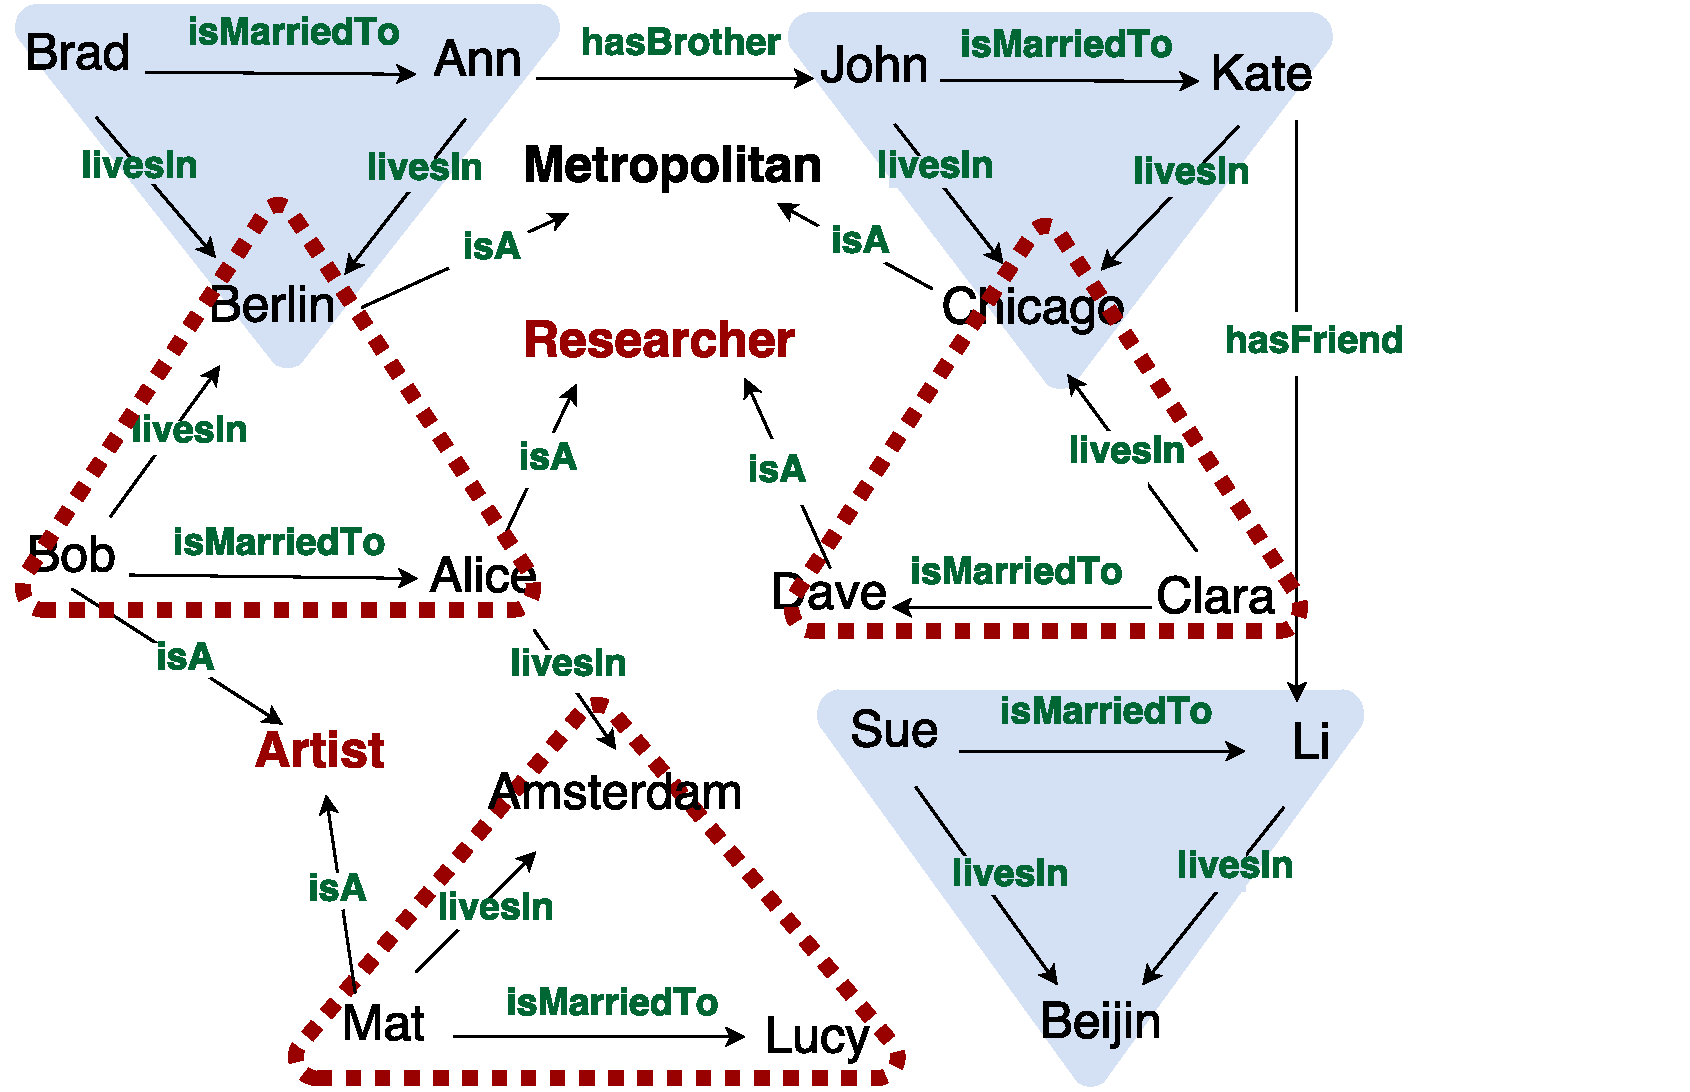
\includegraphics[width=0.7\textwidth]{figures/kg_extended}
\caption{Rule mining for KG completion and KG cleaning}
\label{rdf}
\end{subfigure}
\begin{subfigure}[b]{0.24\textwidth}
\scriptsize
\renewcommand*{\arraystretch}{0.95}
\begin{tabular}{|l|l|l|l|l|l|l|l|l|}
\hline
&  \rot{$\mi{bornInUS}$} &\rot{$\mi{livesInUS}$}&
\rot{$\mi{stateless}$}&\rot{$\mi{immigrant}$}&\rot{$\mi{singer}$}&\rot{$\mi{poet}$}&\rot{$\mi{hasUSPass}$}\\ \hline
$\mi{p1}$ & $\checkmark$ &$\checkmark$ &&&$\checkmark$&&$\checkmark$ \\ \hline
$\mi{p2}$ & $\checkmark$ &$\checkmark$ &&&&&$\checkmark$ \\ \hline
$\mi{p3}$ & $\checkmark$ &$\checkmark$ &&&$\checkmark$&$\checkmark$&$\checkmark$ \\ \hline
$\mi{p4}$ & $\checkmark$ &$\checkmark$ &&&&&$\checkmark$ \\ \hline
$\mi{p5}$ & $\checkmark$ &$\checkmark$ &$\checkmark$&&&& \\ \hline
$\mi{p6}$ & $\checkmark$ & &$\checkmark$&&&& \\ \hline
$\mi{p7}$ & $\checkmark$ & &$\checkmark$&&&& \\ \hline
$\mi{p8}$ & $\checkmark$ & &$\checkmark$&$\checkmark$&&& \\ \hline
$\mi{p9}$ & $\checkmark$ & &&$\checkmark$&&$\checkmark$& \\ \hline
$\mi{p10}$ & $\checkmark$ & &&$\checkmark$&$\checkmark$&$\checkmark$& \\ \hline
$\mi{p11}$ & $\checkmark$ & &&&$\checkmark$&$\checkmark$&$\checkmark$ \\ \hline
\end{tabular}
\smallskip
\caption{US inhabitants KG}
\label{tab:im}
\end{subfigure}
\caption{Examples of Knowledge Graphs}
\end{figure}

Even when meaningful, Horn rules, where all predicates in the rule body are positive such as $\mi{r_1}$ might not always be sufficiently expressive % .
% This is insufficient
to capture KG patterns accurately, as they  cannot handle exceptions, which often appear in practice. 
For instance, application of $\mi{r_1}$ mined from the KG in Figure~\ref{rdf} results in the facts $\mi{livesIn(alice,berlin)}$, $\mi{livesIn(dave,chicago)}$ and $\mi{livesIn(lucy,amsterdam)}$. Observe that the first two facts might be suspected to be wrong. Indeed, both $\mi{alice}$ and $\mi{dave}$ are researchers, and the rule $\mi{r_1}$ could be suspected to have researcher as a potential exception leading to a more accurate rule $\mi{r_2:\;}\mi{livesIn(Y,Z)}\leftarrow \mi{isMarriedTo(X,Y),livesIn(X,Z), not\;researcher(Y)}$.
% Thus making predictions using Horn rules might result in incorrect facts.
% For example, consider a more accurate version of $\mi{r_1}$ given as \\$\mi{r_2{:}livesIn(Y,Z){\leftarrow}
%   isMarriedTo(X,Y){,}livesIn(X,Z){,}{\naf\,} researcher(Y)}$, which \\states that \emph{``Married people live in the same place unless one is a
%   researcher''}. The additional knowledge that Alice is a researcher could be actually an explanation for her living in an unexpected place. If $\mi{r_2}$ often holds, then
% one can no longer complete the missing living place for Dave by assuming that he lives with his wife Clara. 
Exception handling has \\been faced in inductive logic programming (ILP) by learning nonmonotonic logic programs, i.e., programs with negations from databases (e.g., \cite{DBLP:conf/ijcai/InoueK97,DBLP:journals/tocl/Sakama05,R08}), and recently also studied in the context of KGs \cite{gad2016,rumis}.


Unfortunately incompleteness and strong data bias of KGs make the extraction of meaningful rules from them particularly challenging compared to databases that are treated under the Closed World Assumption (CWA, i.e., missing facts are treated as false). Indeed, rules learned from incomplete KGs might be erroneous and might make incorrect predictions on missing facts. 
For example, $\mi{r_3}: \mathit{hasChild(X,Y)}\leftarrow \mathit{worksAt}(X,Z),\mathit{educatedAt}(Y,Z)$ could be mined from a highly incomplete and biased KG stating that workers of certain institutions often have children among the people educated there, 
as this is frequently the case for popular scientists.





Recently, efforts have been put into detecting the concrete numbers of 
facts of certain types that hold in the real world 
(e.g., \emph{``Einstein has 3 children''}) by exploiting Web extraction and crowd-sourcing methods~\cite{cardinality-extraction-iswc-2016,cool-wd}. Such 
meta-data provides a lot of hints about the topology of KGs, and reveals 
parts that should be especially targeted by rule learning methods.
This additional knowledge can be effectively exploited in the rule learning process as shown in \cite{carl}.



The aim of this article is to survey the current research on rule learning from knowledge graphs. We present and discuss different techniques with the roots in inductive logic programming and relational data mining as well as their interalation and applications for KGs. 

\leanparagraph{Tutorial Overview}
In Section~\ref{sec:kgs} we start by briefly introducing knowledge graphs. We then provide neccessary preliminaries on rule-based reasoning over KGs in Section~\ref{sec:reasoning}. Section~\ref{sec:rules_kg_completion} presents an overview of rule learning tasks that can be performed on KGs and describes recent research progress in the context of Horn rule induction. We present techniques for nonmonotonic rule extraction in Section~\ref{sec:nmrulelearn}. Finally, in Section~\ref{sec:discussion_outlook} we conclude the article with an outlook discussion, where we identify a number of promising directions for future work.



\section{Knowledge Graphs(1.5 pages)}
\label{sec:kgs}
Knowledge Graphs (KGs) are large collections of information modeled in the form of entities (such as people, organizations, or places) and the relationships between them. KGs were introduced in the Semantic Web community to create the "web of data" which is readable by machines. This was pushed forward by introducing the W3C Resource Description Framework (RDF)~\cite{rdf2004}. Under this representation entities in the KG are usually encoded as the nodes of the graph and the relations as a directed edges between them~\cite{Nickel2015ARO}. In literature, a simplified representation of KGs as sets of triples in the form of$\tuple{subject, predicate,object}$ (SPO triples, for short) is used. Alternatively, they can also be represented as binary predicate $p(s,o)$, where $subject$ and $object$ are the arguments. 

\begin{example}
The statement \textit{``Christopher Nolan is the director of the science fiction movie Interstellar, which won the Best Visual Effects Oscar"} will be represented in several SPO triples:\\
$\tuple{chris\_nolan, isA, director}$,\\
$\tuple{chris\_nolan, directed, interstellar}$,\\
$\tuple{interstellar, gerne, science\_fiction}$, and \\
$\tuple{interstellar, wonPrize, visual\_effects\_oscar}$.
\end{example}





%about people, organizations, places, etc. Predicates encodes the relations between them, \eg $\tuple{einstein, wasBornIn, Ulm}$. KGs can also be represented similar to formal logic syntax as binary predicate $p(s,o)$, where $subject$ and $object$ are the arguments. KGs can be seen as instantiations for some ontological schema.  
%\leanparagraph{Definition}

\leanparagraph{Construction} KGs are constructed either manually via crowd-sourcing as for \eg Freebase~\cite{Freebase} and Wikidata~\cite{wikidata}, or automatically extracted from semi-structured resources such as Wikipedia, like  YAGO~\cite{yago} and DBpedia~\cite{dbpedia}, or from unstructured resources resulting in KGs such as  NELL~\cite{NELL-aaai15}, KnowledgeVault~\cite{KnowledgeVault}. Table~\ref{tab:kgs}, shows examples for several available KGs (extended discussions can be found in~\cite{Nickel2015ARO,DBLP:journals/semweb/Paulheim17}).


\leanparagraph{KGs quality}

\leanparagraph{Closed World vs. Open World assumptions}

\section{Rules and Reasoning}
\label{sec:reasoning}
In this section we briefly review concepts of logic programming (see \cite{DBLP:conf/rweb/EiterIK09} for more details) and relational association rules \cite{warmer}.

\subsection{Logic Programs} Logic programs consist of a set of rules. Intuitively, a rule is an if-then expression, whose if-part may contain several conditions, some possibly with
negation. The then-part has a single atom that has to hold, whenever the if-part holds. In general, the left part of a rule can also contain disjunctions, but in this tutorial we consider only non-disjunctive rules. More formally,


% Logic rules have been introduced and used in the context of declarative programming. A set of rules are called logical program. There are several types of logical programs (as explained in~\cite{DBLP:books/sp/Lloyd87}), in this tutorial, we are interested in \textit{Horn} and \textit{Nonmonotonic} Logic Programs.

%We define a logic programs similar to~\cite{DBLP:books/sp/Lloyd87}. 
% Similar to ~\cite{DBLP:books/sp/Lloyd87}, we define a \emph{(nonmonotonic) logic program} $P$ is a set of \emph{rules} of the form

\begin{definition}[Rule] A \emph{rule} $r$ is an expression of the form
\begin{equation}
H\leftarrow B, \naf\ E
\end{equation}
where $H$ is a standard first-order atom of the form $a(\vec{X})$, $B$ is a conjunction of positive atoms of the form $b_1(\vec{Y_1}),\dotsc,b_k(\vec{Y_k})$, and $\naf\ E$ %with slight abuse of notation, 
 is a conjunction of negated atoms $\naf\, b_{k+1}(\vec{Y_{k+1}}),\dotsc,\naf\, b_n(\vec{Y_{n}})$. Moreover,  $\vec{X},\vec{Y_1},\ldots,\vec{Y_{n}}$ are tuples of either constants or variables whose length corresponds to the arity of the predicates $a,b_1,\ldots,b_n$ respectively.
% . such that $\naf$ is the so-called \emph{negation as failure (NAF)} or \emph{default negation}, \ie $\naf\, b_n$ is true if either $b_n$ is false or unknown. 
\end{definition}

The left-hand side of a rule $r$ is referred to as its head, denoted by $\mi{head(r)}$, while the right-hand side is its body $\mi{body(r)}$. The positive and negative parts of the body are respectively denoted as $\mi{body^+(r)}$ and $\mi{body^-(r)}$. A rule $r$ is called \emph{positive} or
\emph{Horn} if $\mi{body^-}(r)=\emptyset$.

\begin{example}
Consider $\mi{r_2}$ from Section~\ref{sec:intro}. We have that $\mi{head(r_2)}=\{livesIn(Y,Z)\}$, while $\mi{body^+(r_2)=\{isMarriedTo(X,Y), livesIn(X,Z)\}}$, and moreover it holds that, $\mi{body^-(r_2)=\{not\;researcher(Y)\}}$. \qed
\end{example}


% such that $\vec{X}$, $Y_i$  are vectors of variables and constants with lengths $n$ and $m_i$ respectively. 
 
%$H$ is also known as the rule head and denoted as $\mi{Head(r)}$, $B$ as the positive part of the rule body $\mi{Body^+}(r)$; while, the negated part of the body ($\naf E$) is denoted as $\mi{Body^-}(r)$. 


 % For a program $P$ to be a \textit{Horn logic program}, every $r \in P$ should be \emph{positive} or \emph{Horn}. 
  
  


%Nonmonotonic logical programs are used under the answer set semantics to derive stable models over the given factual knowledge and rules. While, the answer set semantics for nonmonotonic logic programs is based on the CWA, \ie whatever can not be derived from a program is assumed to be false; Nonmonotonic logic programs are widely applied for formalizing common sense reasoning from incomplete information.
%\gad{I commented out the details of answer set semantics (\ie grounding and more)}

A logic program $P$ is \emph{ground} if it consists of only ground rules, i.e. rules without
variables. 

\begin{example}
For instance, a possible grounding of the rule $\mi{r_2}$ is given as follows $\mi{livesIn(dave,chicago)\leftarrow livesIn(clara,chicago),isMarriedTo(clara,dave),}$\\$
\phantom{livesIn(dave,chicago)\leftarrow}\naf\mi{\;researcher(dave)}$. \qed
\end{example}

Ground instantiation $Gr(P)$ of a nonground program $P$ is obtained by substituting variables with constants in all possible ways. 


\begin{definition}[Herbrand Universe, Base, Interpretation]
A \emph{Herbrand universe}  $\mi{HU(P)}$ is a set of all constants occurring in the given program $\mi{P}$. A \emph{Herbrand base}  $\mi{HB(P)}$ is a set of all possible ground atoms that can be formed with predicates and constants appearing inam $P$. A \emph{Herbrand interpretation} is any subset of $\mi{HB(P)}$.
\end{definition}

 By $\mi{MM(P)}$ we denote the set-inclusion minimal Herbrand interpretation of a ground positive program $P$.
\begin{definition}[Gelfond-Lifschitz reduct, answer set]
An interpretation $I$ of $P$ is an \emph{answer set} (or \emph{stable model}) of $P$ iff $I \in \mi{MM}(P^I)$, where $P^I$ is the \emph{Gelfond-Lifschitz (GL) reduct} of $P$, obtained from $Gr(P)$ by removing (i) each rule $r$ such that $\mi{Body}^-(r) \cap I\neq\emptyset$, and (ii) all the negative atoms from the remaining rules. The set of answer sets of a program $P$ is denoted by $AS(P)$.
\end{definition}
%
% \begin{example}
% Consider the program \\
% {\small \leftline{$P = \left\{
%             \renewcommand{\arraystretch}{1.1}
%             \begin{array}{@{\,}l@{~~}l@{}}
%               \mbox{(1) }\mi{bornInUS(alex)};\;\mbox{(2) }\mi{bornInUS(mat)};\;\mbox{(3) }\mi{immigrant(mat)};\\
%               \mbox{(4) } \mi{livesInUS(X)}\leftarrow \mi{bornInUS(X)},  \naf\ \mi{immigrant(X)}\\
%             \end{array}%
%             \!\right\}$}}
            
% \normalsize
% {\smallskip

% \noindent            
% The ground instantiation $Gr(P)$ of $P$ is obtained by substituting $X$ with $\mi{mat}$ and ${alex}$. For $I{=}\{${\small$\mi{bornInUS(alex){,}bornInUS(mat){,}immigrant(mat){,}livesInUS(alex)}$}$\}$, the GL-reduct $P^I$ of $P$ contains the rule $\mi{livesInUS(alex)\leftarrow bornInUS(alex)}$ and the facts (1)-(3). As $I$ is a minimal model of $P^I$, it  is an answer set of $P$.}\qed
% \end{example}
\begin{example}\label{ex:as}
Consider the program \\
{\small \leftline{$P = \left\{
            \renewcommand{\arraystretch}{1.1}
            \begin{array}{@{\,}l@{~~}l@{}}
              \mbox{(1) }\mi{livesIn(brad,berlin)};\;\mbox{(2) }\mi{isMarriedTo(brad,ann)};\\
              \mbox{(3) } \mi{livesIn(Y,Z)\leftarrow isMarriedTo(X,Y),livesIn(X,Z),  \naf\ researcher(Y)}\\
            \end{array}%
            \!\right\}$}}
            
\normalsize
{\smallskip

\noindent            
The ground instantiation $Gr(P)$ of $P$ is obtained by substituting $X,Y,Z$ with $\mi{brad, \,ann}$ and $\mi{berlin}$ respectively. For $I{=}\{${\small$\mi{isMarriedTo(brad{,}ann){,}livesIn(ann{,}berlin)},\\ \mi{livesIn(brad,berlin)}$}$\}$, the GL-reduct $P^I$ of $P$ contains $\mi{livesIn(ann,berlin)}\leftarrow \mi{livesIn(brad,berlin),isMarriedTo(brad,ann)}$ and the facts (1), (2). As $I$ is a minimal model of $P^I$, it holds that $I$ is an answer set of $P$.}\qed
\end{example}
\normalsize

The answer set semantics for nonmonotonic logic programs is based on the CWA, under which whatever can not be derived from a program is assumed to be false. Nonmonotonic logic programs are widely applied for formalizing common sense reasoning over incomplete information.
\subsection{Association Rules}
%\leanparagraph{ mining} 



An association rule is a rule where certain properties of the data in the body of
the rule are related to other properties in its head. For an example of an association rule, consider a
database containing transactional data from a store selling computer equipment.
From this data the association rule stating that 70\% of the customers
buying a laptop also buy a docking station. The knowledge that such rule reflects 
can assist in planning store layout or to decide which customers are likely to respond to an
offer.

Traditionally, the discovery of association rules  has been performed on data stored in a single table.
Recently, however, many methods for mining relational, i.e., graph-based data have been
proposed (see Section~\ref{sec:rules_kg_completion} for details). 

The notion of multirelational association rules is heavily based on frequent conjunctive queries and query subsumption \cite{warmer}. 

\begin{definition}[Conjunctive Query]
A \emph{conjunctive query} $Q$ over a knowledge graph $\cG$ is of the form $Q(\vec{X}):-p_1(\vec{X1}),\dotsc,p_m(\vec{X_m})$. Its  right-hand side (i.e., body) is a finite set of possibly negated atomic formulas over $\cG$, while the left-hand side (i.e., head) is a tuple of variables occurring in the body. The \emph{answer} of $Q$ on $\cG$ is the set $Q(\cG):=\{f(\vec{Y})\,|\,\vec{Y}\,\text{  is the head of } Q \text{ and } f \text{ is a matching of } Q \text{ on } \cG\}$.
\end{definition}

The \emph{(absolute) support} of a conjunctive query $Q$ in a KG $\cG$, is the number of distinct tuples in the answer of $Q$ on $\cG$ \cite{DBLP:conf/ilp/DehaspeR97}. 

\begin{example}
The support of the query
\begin{equation}\mi{Q(X,Y,Z):-marriedTo(X,Y),\, }\mi{livesIn(X,Z)}
\end{equation}
over $\cG$ in Figure~\ref{rdf} asking for people, their spouses and living places is $6$.
\end{example} 
Formally, an \emph{association rule} is of the form $Q_1 => Q_2$, such that $Q_1$ and $Q_2$ are both conjunctive queries and the body of $Q_1$ considered as a set of atoms is included in the body of $Q_2$,  i.e., $Q_1(\cG')\subseteq Q_2(\cG')$ for any possible KG $\cG'$. 

For example, from the above $Q(X,Y,Z)$ and
\begin{equation}Q'(X,Y,Z):-\mi{marriedTo(X,Y),\,livesIn(X,Z),\,} \mi{livesIn(Y,Z)}
\end{equation} we can construct the rule $Q => Q'$. 
 

Association rules are sometimes exploited for reasoning purposes, and thus (with some abuse of notation) can be treated as logical rules, i.e., for $Q_1=>Q_2$ we write $Q_2\backslash Q_1 \leftarrow Q_1$, where $Q_2 \backslash Q_1$ refers to the set difference between $Q_2$ and $Q_1$ considered as sets. For example, $Q=>Q'$ from above corresponds to $\mi{r1}$ from Section~\ref{sec:intro}.

A large number of various measures for evaluating the quality of association rules and their subsequent ranking have been proposed, e.g., \emph{support, confidence}. % The latter is accepted to be appropriate for estimating the actual implication of the rule at hand, and is thus particularly attractive for predictive purposes.

For $r:\;\mi{H\leftarrow B, \naf\ E}$, with $H=\mi{h(X,Y)}$ and $B,E$ involving variables from $\vec{Z}\supseteq X,Y$ and a KG $\cG$, the \emph{standard confidence} (or \textit{confidence}) is given as:\vspace{-.26cm}
\begin{align*}
conf(r,\cG)= \frac{\textit{r-supp}(r,\cG)}{\textit{b-supp}(r,\cG)}
\end{align*}
where $\textit{r-supp}(r,\cG)$ and $\textit{b-supp}(r ,\cG)$ are the \textit{rule support} and \textit{body support}, respectively, which are defined as follows:
\begin{align*}
\textit{r-supp}(r,\cG) &= \#(X,Y): H \in \cG, \exists \vec{Z}\;B\in \cG,E \not \in \cG\\
\textit{b-supp}(r,\cG) &= \#(X,Y):\exists \vec{Z}\; B\in \cG, E \not \in \cG
\end{align*}
\begin{example}
Consider the example rules $\mi{r_1}$, $\mi{r_2}$, and the KG $\cG$ in Figure \ref{rdf}, we have $\textit{r-supp}(r_1,\cG) = \textit{r-supp}(r_2,\cG) = 3$, $\textit{b-supp}(r_1,\cG) = 6$ and $\textit{b-supp}(r_2,\cG) = 4$.
Hence, $\mi{conf(r_1,\cG) = \frac{3}{6}}$ and $\mi{conf(r_2,\cG) = \frac{3}{4}}$.\qed
\end{example}
%\begin{equation}
%\mi{conv(r, \cG)= \dfrac{1 - supp(h(X,Y), \cG)}{1 - conf(r, \cG)}}
%\end{equation}
%where $\mi{supp(h(X,Y),\cG)}$ is the \textit{relative support} of $\mi{h(X,Y)}$ defined as follows:
%\vspace{-.28cm}
%\begin{equation}
%supp(h(X,Y),\cG)=\dfrac{\#(X,Y):h(X,Y)\in \cG}{(\#X:\exists Y\;h(X,Y)\in \cG)*(\#Y:\exists X\;h(X,Y)\in \cG)}
%\end{equation}
%and $\mi{conf}$ is the confidence of $r$ given as
%\begin{equation}
%\mi{conf(r,\cG)=\dfrac{\#(X,Y): H \in \cG, \exists \vec{Z}\;B\in \cG,E \not \in \cG}{\#(X,Y):\exists \vec{Z}\; B\in \cG, E \not \in \cG}}
%\end{equation}
%\vspace{-.3cm}
%\begin{example}
%The conviction of the above rule $\mi{r1}$ is $\mi{conv(r1,\cG)}=\dfrac{1-0.3}{1-0.5}=1.4$\qed
%\end{example}

\subsection{Reasoning over KGs} Rule-based reasoning is used for KGs refinement to solve their inaccuracy and incompleteness~\cite{DBLP:journals/semweb/Paulheim17}. KG completion is one of the main reasoning tasks performed on the KG that is concerned with predicting the missing facts in the KG using the rules and currently existing facts. More formally, 



 \begin{definition}[Rule-based KG completion]\label{def:kgcomp} Let $\cG$ be a KG and $\cA$ its factual representation over the signature $\Sigma_{\cG}=\tuple{\cR,\cC}$. Let, moreover, $P$ be a set of rules with predicates from $\cR$. % $\Sigma_{P}=\tuple{\mathbf{C}\cup \mathbf{R},\cC}$
 Then \emph{completion of $\cG$ (resp. $\cA$) \wrt\ $P$} is a graph $\cG_{P}$ constructed from any answer set $\cG_{\cR}\in AS(P \cup \cG)$. 
 \end{definition}
 
 \begin{example}
 Given the KG in Figure~\ref{rdf} as $\cG$ and rule $r_2$ from Section~\ref{sec:intro}, let us assume the rule set $P=\{r_2\}$; thus, the completion of $\cG$ would be $\cG_{P}=\cG \cup \{\mi{livesIn(lucy,amsterdam)}\}$. Not that, predictions such as $\mi{livesIn(alice, berlin)}$ and $\mi{livesIn(dave, chicago)}$ are not part of the answer set (since they both are researchers); and hence, they do not belong to the complete graph $\cG_{P}$ .
 \end{example}

% \leanparagraph{KG cleaning}

% \leanparagraph{KG completion} In this task rules are used to predict the missing facts in the KG based on the existing facts in the knowledge graph. This can be formally defined as:


\section{ Rule Learning for Knowledge Graph Completion}
\label{sec:rules_kg_completion}
\subsection{Rule Learning Tasks}
Rule learning is an important subfield of machine learning research area, which focuses on symbolic methods for intelligent data analysis. Here by symbolic, we mean methods that employ some kind of description language in which the learned knowledge is expressed. One of the main attractions of rule induction is that the rules are much more transparent and easier to interpret that, e.g., a regression model or trained neural network.

First-order learning approaches are also referred to as \emph{relational data mining (RDM)}, \emph{relational learning
(RL)} or \emph{inductive logic programming (ILP)}, as the patterns they discover are expressed in
relational formalisms of first-order logic.

Rule learning approaches can be characterized along several dimensions. 
\begin{itemize}
\item \emph{type of the data source}, e.g., KG, database, text, oracle (a domain expert), true and false facts over a certain target predicate (i.e., so-called positive and negative examples respectively)
\item \emph{type of the output knowledge}, e.g., Horn rules, nonmonotonic rules, description logic class descriptions, class inclusions of various expressivity, etc.
\item \emph{method used}, e.g., natural language processing, machine learning, association rule mining, theory revision, oracle-based exact learning techniques, etc.
\item \emph{data (in)completeness assumption}, e.g., OWA, CWA, partial completeness assumption, etc.
\item \emph{availability and type of background knowledge}, e.g., DL ontology, set of datalog rules.
\end{itemize}

In this work we focus on approaches that rely on \emph{relational association rule learning} and \emph{theory revision} techniques for extraction of \emph{Horn} and \emph{nonmonotonic rules} respectively from incomplete KGs treated under OWA. Moreover, we discuss exploitation of additional \emph{background knowledge} in the form of constraints on the missing edge counts.

Association rule mining concerns the discovery of frequent patterns in a data set and the subsequent transformation of these patterns into rules. Association rules in the relational format have been subject of intensive research in ILP (see, e.g., \cite{DBLP:conf/ilp/DehaspeR97} as the seminal work in this direction). In the following we adapt basic notions in relational association rule mining to our case of interest.

\subsection{Rule Construction Methods}
Traditional rules learning systems in the context of Inductive Logic Programming (ILP) \cite{probfoil,DBLP:conf/ijcai/RaedtDTBV15,DBLP:conf/clima/CorapiSIR11} are either memory-expensive or requires the availability of negative examples, which is hard to get due to the large KG size. In contrast, other unsupervised relational 
association rule learning systems deduce logical rules from the KG by mining frequent patterns and casting them into implications. Most of the  existing methods tailored towards Open World Assumption (OWA) rely only on the available graph and exploit sophisticated rule measures \cite{amie,op,rumis}.
In this section, we briefly summarize some of these state-of-the-art rule mining systems, which combine rule learning and reasoning for knowledge graph completion under OWA. We classify them into two main categories: Horn rules learning and Non-monotonic rules learning systems.
Horn rule learning systems focus on mining rules consisting of only positive atoms. Most of these systems only extract rules that are \emph{closed}, where every variable appears at least twice. Some examples of such mining systems are AMIE \cite{amie}, OP, \cite{op} and RDF2Rules \cite{rdf2rules}.
\subsubsection{AMIE.}
AMIE \cite{amie} is a state-of-the-art positive rule mining system in the context of OWA. 
%Apart from the algorithm being used to construct rules, AMIE also introduces a novel rule measure namely PCA confidence, which is based on the Partial Closed world Assumption (PCA), stating that data of the knowledge graph is added in batch \cite{amie}. In particular, with every $p(s,o) \in \cG$, the assumption states that:
%\[\forall o' : p(s,o') \in \cG^i \Rightarrow p(s,o') \in \cG\]
%Intuitively, if the KG contains some $p$-object of $s$, then it also contains all possible $p$-objects of $s$. Formally, PCA confidence is defined as follows:\thi{pca conf here}
%\[conf_{pca}=.\]
%This measure is then exploited by AMIE to mine positive rules using its introduced algorithm. 
In AMIE, rule is treated as a sequence of atoms, where the first atom is the head of the rule, and other atoms are the body of the rule. Mining operators are introduced to extend the sequences of atoms to explore the rules' search space as follows:
\begin{itemize}
\item \textit{Add Dangling Atom}: This operator adds a positive atom to the rule. One of the two arguments of the atom should be a fresh new variable. The other argument is a shared variable, which appears in some other atom of the rule.
\item \textit{Add Instantiated Atom}: This operator adds a positive atom to the rule, in which one argument of the atom is constant (entity) and the other argument is a shared variable with the rule.
\item \textit{Add Closing Atom}: This operator adds a positive atom to the rule, in which both arguments of the atom are shared variables with the rule.
\end{itemize}
\begin{algorithm}[t]
\DontPrintSemicolon
$queue\leftarrow \langle[]\rangle$\\
Execute in parallel:\\
\While{$\neg$queue.isEmpty()}{    
    \textit{rule $\leftarrow$ queue.dequeue()}\\
%    \tcc{Computes rule statistics and output if necessary.}
    \If{rule.isClosed()}{
        \eIf{rule is not pruned for outputting}{
            output($rule$)
        }{
            continue while loop
        }
    }
%    \tcc{Applies operators to explore more new rules.}
    \ForEach{operator o}{
        \ForEach{newRule $\in$ o(rule)}{
%            \If{newRule.hasGoodFormat()}{
%                \tcc{Check whether there exists some version of the rule in queue.}
                \If{newRule $\notin$ queue}{ 
                    \textit{queue.enqueue(newRule)}
%               }
            }
        }
    }    
}
\caption{AMIE's mining algorithm.}
\label{algor:amie}
\end{algorithm}
Algorithm \ref{algor:amie} presents how AMIE's algorithm applies mining operators to extract rules from KGs. The algorithm maintains a queue consisting of rules to be processed. At the beginning, the queue contains only an empty rule. At each step, one rule is taken from the head of the queue, then being checked for outputting. Then, mining operators are applied to explore new more rules.
Checking for outputting is the process of collecting rules' statistics including: support, PCA confidence, head coverage, and then checking whether these metrics pass some defined threshold. Apart from that, the expansion of rules must meet the other two requirements: the increasing of rule's quality, and the language bias. In particular, firstly, adding an atom into the rule must increase its quality (AMIE uses PCA confidence). Secondly, the rule must be \textit{closed} and number of atoms of the rule does not exceed some threshold.

To computing rule's statistics, we must find all instances of rule's variable in the KG. Several options have been proposed by AMIE depending on how the KGs are stored: either by using SQL, SPARQL \cite{amie} or using an In-Memory Database.

\subsubsection{RDF2Rules.}
While AMIE mines one rule at a time, RDF2Rules \cite{rdf2rules} parallelizes this process by first extracting Frequent Predicate Cycles (FPCs) of some length $k$, which have the following form:
\[\theta = (x_1, p_1^{d_1}, x_2, p_2^{d_2}, ..., p_k^{d_k}, x_1)\]
where, $x_i$s are variables to be appeared in the rules, $p_i$s are predicates between these variables, and $d_i$s $\in \{0,1\}$ state the direction of these predicates. Then, rules are extracted from the FPC by choosing a predicate as the head, and other predicates into the body of the rule. Formally, rule $j$-th is generated from the FPC as follows:
\[r_j: p_j^{d_j}(x_j,x_{j+1}) \leftarrow \underset{i \in [1,k], i \ne j}{\bigwedge} p_i^{d_i}(x_i,x_{i+1}) \]

Moreover, RDF2Rules is also capable of generating rules with $type$ information. The above generated rules are without \textit{type} information. To achieve this, each extracted FPC will be enhanced with frequent types of variables. These information could be then added to the body of each generated rule. Nevertheless, comparing to AMIE, even though RDF2Rules can mine rules faster, the forms of rule it can learn are restricted, since the rules extraction strictly relies on FPCs.

\subsubsection{OP (Ontological Pathfinding).} 
Learning rules from knowledge graph consists of two phases: constructing the rules and examining their quality based on the KG. Most of state-of-the-art rule mining systems parallelize only the construction of the rules, while the quality of the rules are determined by a single thread.
Modern web-scale knowledge bases such as YAGO or Freebase might contain hundreds million of entities and billions of facts between them, Hence, it is impossible to store these KGs in a single machine. As a result, these rule mining systems either cannot scale to this size to determine the rules' quality, or they have to assign this task to some third-party system such as SQL, SPARQL \cite{amie}, which might be inefficient.

The focus of the novel rule-mining algorithm OP\cite{op} is not at how to find the candidate rules in the knowledge graph, but rather at how to examine their quality. The rules construction in Ontological Pathfinding (OP) algorithm relies on the relational pathfinding method \cite{DBLP:conf/aaai/RichardsM92}. The only difference is that, instead of finding paths on the entity-relations graph, OP looks at the domain-range schema graph \cite{op}. After candidate rules are constructed, their quality is determined via a sequences of parallelization and optimization methods including partitioning, joining and pruning strategies. 
\subsection{Rule Evaluation}
Most of state-of-the-art positive rule mining systems are different from each other at the rule metric that they introduce to quantify rule's quality and how to exploit it in learning rules. Basically, we can plug different rule metrics into these mining systems to work under different situations. For instance, standard confidence $conf$ and PCA confidence $conf_{pca}$ works under the Closed World Assumption and the Partial Completeness Assumption, correspondingly. Apart from that, there also exist other measures introduced to quantify the quality of rules (see \cite{metrics-summary}). Some of them are listed below.
\subsubsection{Conviction.} Conviction is shown to guarantee the high predictive power \cite{Azevedo2007} by measuring the intensity of rule's implication \cite{metrics-summary}. Given $\mi{r:\; head\leftarrow body^+, not\;  body^-}$, conviction of $r$ is computed as follows:
\begin{align*}
\textit{conv}(r,\cG) & := \frac{1 - \textit{rel-supp}(head, \cG)}{1-\textit{conf}(r,\cG)}
\end{align*}
where $\textit{rel-supp}(head)$ is the relative support of the head measured by:
\begin{align*}
\textit{rel-supp}(head, \cG) = \frac{|\{(h, t) \mid head(h,t) \in \cG\}|}{|\{h \mid \exists t':head(h,t') \in \cG\}| \times |\{t \mid \exists h': head(h',t) \in \cG\}|}
\end{align*}
\subsubsection{PCA Confidence.} Proposed by AMIE \cite{amie}, this measure considers KGs under the Partial Completeness Assumption (PCA), saying that data of the knowledge graph is added in batch \cite{amie}. In particular, with every $p(s,o) \in \cG$, the assumption states that:
\[\forall o' : p(s,o') \in \cG^i \Rightarrow p(s,o') \in \cG\]
Intuitively, if the KG contains some $p$-object of $s$, then it also contains all possible $p$-objects of $s$. Formally, PCA confidence is defined as follows:
\[conf_{pca}(r,\cG) = \frac{supp(r,\cG)}{pr-supp(r,\cG)}\]
\subsubsection{Soft Confidence.} Introduced by RDF2Rules \cite{rdf2rules}, soft confidence is also tailored to work under Open World Assumption, measured by:
\[conf_{st}(p(s,o) \leftarrow B) = \frac{sup(p(s,o) \leftarrow B)}{sup(B) - \sum_{e \in U}P(e,p)} \]
where $U$ is the set of entities that previously have no relations of $p$, but have new predicted relations of $p$ by the rule, and $P(e,p)$ is the probability of entity $e$ having relation $p$, which is approximated by using entity \textit{type} information \cite{rdf2rules}:
\[P(e,p)  = max_{t \in T_e}\frac{|Inst_p(t)|}{|Inst(t)|}{}\]
Here, $T_e$ contains all $type$ of entity $e$, $Inst(t)$ contains all entities having type $t$, and $Inst_p(t)$ is similar to $Inst(t)$, but restricts to only entities that have relation $p$.
Intuitively, soft confidence is designed to avoid the underfitting of standard confidence and overfitting of PCA confidence by also taking into account the probability of entities having the head predicate $P(e,p)$ in the unknown part of the rule.
\subsubsection{Completeness-aware Rule Measures.}  
\begin{figure}[t]
\begin{center}
%\includegraphics[width=.8\textwidth]{figures/fam_grad}

%%%%%% New KG %%%%%%%

\begin{tikzpicture}[->,>=stealth',auto,node distance=3cm,
  thick,main node/.style={font=\bfseries}]

  \node[main node] (1) {john};
  \node[main node] (2) [right=3cm of 1] {mary};
  \node[main node] (3) [below left=1cm and 2cm of 1] {alice};
  \node[main node] (4) [below right=1cm and 1.5cm of 1] {bob};
  \node[main node] (5) [below right=1cm and 2cm of 2] {carol};
  \node[main node] (6) [above left=1cm and 2cm of 1] {dave};
  \node[main node] (7) [above right=1cm and 1.5cm of 1] {tuwien};
  \node[main node] (8) [above right=1cm and 2cm of 2] {mpi};

  \path[every node/.style={color=teal,fill=white,font=\small}]
    (1) edge node [right=-20pt] {worksAt} (7)
    (2) edge node [right=-15pt] {worksAt} (7)
    (4) edge node [right=-30pt] {educatedAt} (7)
    (2) edge node [right=-10pt] {hasChild} (4)
    (2) edge node [left=-20pt] {hasChild} (5)
    (1) edge[bend left=20] node [right=-20pt] {hasChild} (4)
    (4) edge[bend left=20] node [left=-20pt] {hasFather} (1)
    (1) edge[bend right=20] node [right=-20pt] {hasChild} (3)
    (3) edge[bend right=20] node [right=-20pt] {hasFather} (1)
    (2) edge node [left=-20pt] {educatedAt} (8)
    (5) edge[bend left=20] node [left=-10pt] {educatedAt} (8)
    (5) edge[bend right=20] node [right=-10pt,pos=0.4] {worksAt} (8)
    (6) edge node [right=-5pt] {hasFather} (1)
    (3) edge[bend right=20] node [right=-10pt,pos=0.55] {hasSibling} (6)
    (6) edge[bend right=20] node [left=-10pt,pos=0.65] {hasSibling} (3)
    (6) edge[bend left=20] node [above=-10pt] {worksAt} (7)
    (6) edge[bend right=5] node [below=-10pt] {educatedAt} (7)
    (4) edge node [right=-20pt] {hasSibling} (5)
    ;
\end{tikzpicture}

\caption{Example KG}
\label{fig:fam_grad}
\end{center}
\end{figure}

In the solutions for the rule-based KG completion problem discussed so far, no external meta-information from outside of the KG about potential existence of certain types of facts was exploited. However, this knowledge is obviously useful, and furthermore, it is even available on the Web
in the form of Cardinality Statements, e. g., Brad has three children or Mary is a citizen of two countries. If a given KG mentions just a single Brad’s child, we could be aiming at extracting rules that predict the missing
one. Since such existential information is beneficial not only for guided rule learning but also for increasing the scope of KGs and estimating their recall.

Thus, recent work CARL \cite{carl} focused on the improvements of rule scoring functions by making use of these extra (in-)completeness meta-data.

Overall, for a given fact $\tuple{john, hasChild, mary}$, CARL takes into account the following two numerical statements: the number of (1) children of $john$ and (2) incoming edges to $mary$, which in practice can be obtained using web extraction techniques \cite{cardinality-extraction-iswc-2016}. Since template (2) could be rewritten as the instances of the template (1) through the inverse relations, these meta-data statements could be formalized as follows:
\[\mi{num}(p,s) = \# o : p(s,o) \in \cG^i\]
indicating the total number of objects $o$ for a given subject $s$ and predicate $p$. Based on this, the number of missing objects $o$ in the available graph $\cG$ can be retrieved:
\[\mi{miss}(p,s) = \mi{num(p,s)} - \#o : p(s,o) \in \cG\]
Given a KG and its related cardinality statements of the above form, CARL defines two indicators for each given rule $r: %\vec{H}
\mi{h(X,Y)}\leftarrow \vec{B}$, %with $\vec{H}=h(X,Y)$, 
reflecting the number of new 
predictions made by $\mi{r}$ in incomplete ($\mi{npi(r)}$) and, respectively, complete ($\mi{npc(r)}$) KG parts:
\begin{align*}
\mi{npi}(r) = \sum_x min(\#y: h(x,y)\in \cG_r\backslash \cG, \mi{miss}(h,x))
\end{align*}
\vspace{-\topsep}
\vspace{-\topsep}
\begin{align*}
\mi{npc}(r) = \sum_x max(\#y: h(x,y)\in\cG_r\backslash \cG - \mi{miss}(h,x), 0)
\end{align*}
Using these indicators, a class of completeness-aware rules measures have been proposed by CARL as follows:
\begin{itemize}
\item \textbf{Completeness Confidence.} First, incompleteness information is used to determine whether to consider an instance in the unknown part of the rule as a counterexample or not. Formally, the \emph{completeness confidence} is defined as follows:
\begin{align*}
\mi{conf_{comp}}(r) := \frac{\mi{supp}(r)}{\mi{supp}(\vec{B}) - \mi{npi}(r)}
\end{align*}
\item \textbf{Completeness Precision and Recall.} In the spirit of information retrieval, the notions of \emph{completeness precision} and \emph{completeness recall} are defined to measure rule quality based on their predictions in complete and incomplete KG parts:
\begin{align*}
\mi{precision_{comp}}(r)=1-\frac{\mi{npc}(r)}{\mi{supp}(\vec{B})},\;\;\;\;\; \mi{recall_{comp}}(r)=\frac{\mi{npi}(r)}{\sum_s \mathit{miss}(h,s)}
\end{align*}
Intuitively, rules having high precision are rules that predict few facts in complete parts, while rules having high recall are rules that predict many facts in incomplete ones. Rule scoring could also be based on any weighted combination of these two metrics.
%The \emph{recall measure} is similar to classical support measures, but now expresses how many facts on KG parts known to be incomplete, are generated by the rule (the more the better). The \emph{precision measure}, in turn, assesses how many of the generated facts are definitely wrong, namely those in complete parts (the more of these, the worse the rule). In fact, this is an upper bound on the precision, as the other facts cannot be evaluated.
\item \textbf{Directional Metric.} If rule mining does make use of completeness information, and both do not exhibit any statistical bias, then intuitively the rule predictions and the (in)complete areas should be statistically independent. On the other hand, correlation between the two indicates that the rule-mining is \emph{(in)completeness-aware}. Hence, \emph{directional metric} is proposed following this intuition by measuring the proportion between predictions in complete and incomplete parts:
\begin{align*}
\mi{dm}(r) := \frac{\mi{npi}(r)-\mi{npc}(r)}{2\cdot(\mi{npi}(r)+\mi{npc}(r))}+0.5
\end{align*}
Since the real-world KGs are often highly incomplete, it might be reasonable to put more weight on predictions in complete parts. This can be done by multiplying predictions made in complete parts by a certain factor. This leads to the consideration of the weighted combination of a existing association rule measure, e.g., standard confidence or conviction, and 
the directional metric, using a weighting factor $\beta \in [0..1]$. With standard confidence, we obtain:
\begin{align*}
\mi{weighted\_dm}(r)=\beta \cdot \mi{conf}(r) + (1-\beta) \cdot \mi{dm}(r) 
\end{align*}
\end{itemize}
%%Recent works, e.g., \cite{cardinality-extraction-iswc-2016} focused on the task of extracting such cardinality information from text.We now discuss possible ways of making use of such information in rule scoring and ranking, which are core steps in association rule learning. A variety of measures for ranking rules have been proposed, with prominent ones being confidence, conviction and lift.  The existing (in-)completeness-aware rule measure in the KG context (the PCA confidence \cite{amie}) has two apparent shortcomings: First,  it only counts as counterexamples those %objects pairs $(x,y)$ for which at least one $h(x,y')$ %other facts 
%%with the head predicate $\mi{h}$ 
%%holds is in $\cG^a$ for some $\mi{y'}$ and a rule's head predicate $h$. This means it may incorrectly give high scores to rules predicting facts for very incomplete relations, e.g., \emph{place of baptism}. Second, it is not suited for data in non-functional relations that is not added in batches, such as awards, where the important ones are added instantly, while others much slower or even possibly never. 
%
%
%%Before dwelling into the details of our approach we discuss the formal representation of such meta-data. 
%
%%\leanparagraph{Cardinality Statements}
%%Overall, one can think of 6 different cardinality templates obtained by fixing subject, predicate or object in a triple and report the number of respective facts that hold in $\cG^i$. 
%%The lattice of possible basic (in)completeness templates on the fact level is presented in Fig.~\ref{fig:cs} 
%%on an example triple $\langle\mi{john\;hasChild\;mary}\rangle$. By fixing subject, predicate or object in a triple overall we obtain 6 different templates.
% %statements for these templates 
%% Ideally, we would be willing to possess and exploit numerical statements for all of these templates. For example,
%E.g., for $\mi{\tuple{john\;hasChild\;mary}}$ we %can construct the following cardinality assertions: 
%can count
%(1) children of $\mi{john}$ %has $\mi{n}$ children; 
%(2) edges from $\mi{john}$ to $\mi{mary}$; % there are $n$ edges; 
%(3) incoming edges to $\mi{mary}$; % has $n$ incoming $\mi{hasChild}$ edges; 
%(4) %there are $\mi{n}$ 
%facts with $\mi{john}$ as a subject; (5) %there are $n$ 
%facts over $\mi{hasChild}$ relation; (6) %there are $\mi{n}$ 
%facts with $\mi{mary}$ as an object. 
%
%In practice, numerical statements for templates (1) and (3) can be obtained using web extraction techniques \cite{cardinality-extraction-iswc-2016}, from functional properties of relations or from crowd-sourcing. For other templates things get trickier; one might be able to learn  
%them from the data or they could be defined by domain experts in topic-specific KGs. We leave this issue for future work, and focus here only on templates (1) and (3), which could be rewritten as the instances of the template (1) provided that inverse relations can be expressed in a KG. For instance, $\# s: \mi{hasChild}(s,\mi{john})=\# o: \mi{hasParent}(\mi{john},o)$ for the predicates $\mi{hasChild}$ and $\mi{hasParent}$, which are %in an 
%inverses of one another. % relation. 
%
%We represent the (in)completeness meta-data using cardinality statements by reporting (the numerical restriction on) the absolute number of facts over a certain relation in the ideal graph $\cG^i$. More specifically, we define the partial function $num$ that takes as input a predicate $\mi{p}$ and a constant $\mi{s}$ and outputs a natural number corresponding to the number of facts in $\cG^i$ over $\mi{p}$ with $\mi{s}$ as the first argument: 
%
%\begin{equation}\label{eq:num}
%\mi{num}(p,s) := \# o : p(s,o) \in \cG^i 
%\end{equation}
%
%Naturally, the number of missing facts for a given $p$ and $s$ can be obtained as
%
%\begin{equation}\label{eq:miss}
%\mi{miss}(p,s) := \mi{num(p,s)} - \#o : p(s,o) \in \cG^a %\setminus \cG^a
%\end{equation}
%
%\begin{example}
%\label{ex:cardinality}
%Consider the KG in Fig.~\ref{fig:fam_grad}.
%%and the rules $\mi{r1}$ and $\mi{r_2}$ from Example~\ref{ex:conf},
%%along with the following 
%%The following 
%and the following cardinality statements for it: %it might be available:
%\vspace{-\topsep}
%\begin{itemize}
%\setlength{\parskip}{0pt}
%\setlength{\itemsep}{0pt plus 1pt}
%\item $\mi{num(hasChild,john)}\!=\!\mi{num(hasChild,mary)}\!=3$; $\mi{num(hasChild,alice)}\!=\!1$;\\  $\mi{num(hasChild,carol)}\!=\!\mi{num(hasChild,dave)}\!=\!0$;
%\item $\mi{num(hasSibling,bob)}\!=\!3$;
%      $\mi{num(hasSibling,alice)}\!=\!\mi{num(hasSibling,carol)}\!=\!\mi{num(hasSibling,dave)}\!=\!2$.
%\end{itemize}
%\vspace{-\topsep}
%We then have:
%\vspace{-\topsep}
%\begin{itemize}
%\setlength{\parskip}{0pt}
%\setlength{\itemsep}{0pt plus 1pt}
%\item $\mi{miss(hasChild,mary)}\!=\!\mi{miss(hasChild,john)}\!=\!\mi{miss(hasChild,alice)}\!=\!1$;\\
%      $\mi{miss(hasChild,carol)}\!=\!\mi{miss(hasChild,dave)}\!=\!0$; 
%\item $\mi{miss(hasSibling,bob)}\!=\mi{miss(hasSibling,carol)}\!=\!2$;\\ 
%      $\mi{miss(hasSibling,alice)}\!=\!\mi{miss(hasSibling,dave)}\!=\!1$.\qed
%\end{itemize}
%\end{example}
%
%
%We are now ready to 
%define the \emph{completeness-aware rule scoring problem}.
%%\begin{problem}[Completeness-aware rule scoring] 
%Given a KG and a set of 
%%(in-)-complete\-ness
%cardinality statements, \emph{completeness-aware rule scoring} aims to score rules not only by their predictive power on the known KG, but also wrt.\ the number of wrongly predicted facts  
%in complete areas and the number of newly predicted 
%facts in known incomplete areas.
%%\end{problem}
%
%In the following we discuss and compare  
%three novel approaches for completeness-aware rule scoring. These are (i) the \emph{completeness confidence}, (ii) \emph{completeness precision} and \emph{recall}, 
%and (iii) \emph{directional metric}.
%Henceforth, all examples 
%consider the KG in Fig.~\ref{fig:fam_grad}, 
%rules from Ex.~\ref{ex:conf}, and cardinality statements  described in Ex.~\ref{ex:cardinality}.
%
%\leanparagraph{Completeness Confidence} In this work we propose to explicitly rely on incompleteness information in determining whether to consider an instance as a counterexample for a rule at hand or not.
%
%To do that, we first define two indicators for  a given rule $r: %\vec{H}
%\mi{h(X,Y)}\leftarrow \vec{B}$, %with $\vec{H}=h(X,Y)$, 
%reflecting the number of new 
%predictions made by $\mi{r}$ in incomplete ($\mi{npi(r)}$) and, respectively, complete ($\mi{npc(r)}$) KG parts:
%
%
%
%\begin{equation}
%\mi{npi}(r) := \sum_x min(\#y: h(x,y)\in \cG^a_r\backslash \cG^a, \mi{miss}(h,x))
%\end{equation}
%\vspace{-\topsep}
%\begin{equation}
%\mi{npc}(r) := \sum_x max(\#y: h(x,y)\in\cG^a_r\backslash \cG^a - \mi{miss}(h,x), 0)
%\end{equation}
%
%Note that summation is done exactly over those entities for which $\mi{miss}$ is defined.
%Exploiting these additional indicators 
%for %a given 
%$r:\,h(X,Y)\leftarrow \vec{B}$ we obtain the following \emph{completeness-aware confidence}:
%
%\begin{equation}\label{eq:comp_conf}
%\mi{conf_{comp}}(r) := \frac{\mi{supp}(r)}{\mi{supp}(\vec{B}) - \mi{npi}(r)}
%\end{equation}
%
%\begin{example}\label{ex:fam_grad}
%\label{ex:conf_comp}
%%Consider the KG in Fig.~\ref{fig:fam_grad}, rules $\mi{r1}$ and $\mi{r_2}$ from Example~\ref{ex:conf}, and cardinality statements mentioned in Example~\ref{ex:cardinality}.
%Obviously, the rule $\mi{r_2}$ %is
%should be preferred over $\mi{r_1}$. For our novel %This desired rule ranking is achieved by exploiting our novel 
%completeness confidence, we get %giving 
%$\mi{conf_{comp}(r_1)}=\frac{2}{6}$ %{5}$ 
%and $\mi{conf_{comp}(r_2)}=\frac{1}{2}$, resulting in the desired rule ordering,  which is not achieved by %is in contrast to 
%existing measures. %while the %previously introduced 
%%The existing %ranking 
%%metrics result in an incorrect rule ordering 
%%(see Ex.~\ref{ex:conf} and~\ref{ex:conf_pca}).
%\qed
%%%%%% OLD EXAMPLE %%%%%
%%\begin{example}\label{ex:fam_grad}
%%Consider the KG in Fig.~\ref{fig:fam_grad} along with the following cardinality statements:\\ $\mi{num(hasChild,mary)=num(hasChild,john)=3,num(hasChild,alice)=0}.$ 
%%Assume that the rules $\mi{r1}$ and $\mi{r_2}$ were mined from this KG.
%
%%\begin{itemize}
%%\item $\mi{r_1:\,hasChild(X,Y)\leftarrow worksAt(X,Z),graduateOf(Y,Z)}$
%%\item $\mi{r_2:\,hasChild(X,Y)\leftarrow hasParent(Y,X)}$;
%%\end{itemize}
%
%%Obviously, rule $\mi{r_1}$ is preferred over $\mi{r_2}$. This desired rule ranking in achieved by exploiting our novel completeness confidence, while the previously introduced ranking metrics result in an incorrect rule ordering.
%%\begin{itemize}
%%\item $\mi{conf(r_1)=2/3,conf(r_2)=2/5}$
%%\item $\mi{conf_{pca}(r_1)=1,conf_{pca}(r_2)=2/5}$
%%\item $\mi{conf_{comp}(r_1)=1/3,conf_{comp}(r_2)=1}$ \qed
%%\end{itemize}
%%%%%%%%%%%%%%%%%%%%%%%%
%
%
%\end{example}
%
%%The proposed metric generalizes %over 
%Our completeness confidence generalizes both 
%the standard %confidence 
%and the PCA confidence:
%
%\begin{proposition}
%For every KG $\cG$ and rule $r$ it holds that 
%\begin{itemize}
%\item[(i)] under the Closed World Assumption (CWA) $\mi{conf_{comp}(r)=conf(r)}$;
%\item[(ii)] under the Partial Completeness Assumption (PCA) $\mi{conf_{comp}(r)=conf_{pca}(r)}$.
%\end{itemize}
%\end{proposition}
%
%\begin{proof}
%\textbf{(i)} Under the CWA, it holds that for all $ p\in \mathbf{R},\,s\in \cC: \mi{miss}(p,s) = 0$. Thus, for all rules $r$, we have that $\mi{npi}(r) = 0$, and hence, $\mi{conf_{comp}(r)}=\mi{conf(r)}$.
%\smallskip
%
%\noindent \textbf{(ii)} Under the PCA, it is assumed that for all $p\in \mathbf{R}$ and $s \in \cC$ it holds that 
%$\mi{miss}(p,s) = 0$ if $\exists o: p(s,o)\in \cG^a$. We extend the PCA by assuming that $miss(p,s)=+\infty$ for KG parts for which cardinality statements are unavailable, which is a reasonable assumption given the overall incompleteness of the available KG, i.e., 
%%and otherwise, 
%$\mi{miss}(p,s) = +\infty$. 
%%, since the number of missing facts is unrestricted. 
%Hence, for all $r$ we have
%$\mi{npi(r)=\sum_{x}predict(r,x)}$, where
%
%\begin{center}
%$predict(r,x)=
%\begin{cases}
%0, \text{ if } \exists y: h(x,y)\in \cG^a\\
%\#y: h(x,y) \in \cG^a_r\backslash \cG^a, \text{ if } \forall y': h(x,y')\not\in \cG^a\\
%\end{cases}$
%\end{center}
%From this we get
%
%\begin{center}
%$\mi{conf_{comp}(r)=\dfrac{supp(r)}{supp(\vec{B})-\sum_{x: \forall y': h(x,y')\not\in\cG^a}\#y: h(x,y)\in \cG^a_r\backslash \cG^a}}$
%\end{center}
%
%The denominator of the latter formula counts all rule body and subtracts from them those, for which the head $h(x,y)$ is predicted and $\forall y':h(x,y')\not \in \cG^a$. Hence, we end up counting only  body substitutions with $h(x,y')\in \cG^a$ for at least  one $y'$, i.e., $\mi{\#(x,y):\exists \vec{Z}:\vec{B}\wedge \exists y': h(x,y')\in \cG^a}$, from which the result follows. \qed
%
%\end{proof}
%
%
%
%In other words, if %we assume that 
%the graph is known to be fully complete, i.e., for all $p \in\cR,s\in\cC$ we have
%$\mi{miss}(p,s)=0$ , then $\mi{conf_{comp}}$ is the same as the standard confidence. Similarly, if  $\mi{miss}(p,s)= 0$ for such $p,s$ pairs that at least one 
%fact $p(s,\_)\in \cG^a$ exists and  $\mi{miss}(p,s) = +\infty$ for the rest,  
%then $\mi{conf_{comp}}$ is the same as the PCA confidence.
%
%\leanparagraph{Completeness Precision and Recall} Further developing the idea of scoring rules based on their predictions in complete and incomplete KG parts, we propose to consider the notions of  \emph{completeness precision} and \emph{recall}\footnote{For brevity we skip the word "completeness" if clear from the context.} for rules defined in the spirit of information retrieval. Intuitively, rules having high precision are rules that predict few facts in complete parts, while rules having high recall are rules that predict many facts in incomplete ones. Rule scoring could then be based on any weighted combination of these two metrics.
%
%Formally, we define the precision and recall of a rule $\mi{r: h(X,Y)\leftarrow \vec{B}}$ as follows:
%
%\begin{equation}\label{eq:precision}
%\mi{precision_{comp}}(r)=1-\frac{\mi{npc}(r)}{\mi{supp}(\vec{B})}
%\end{equation}
%
%\begin{equation}\label{eq:recall}
%\mi{recall_{comp}}(r)=\frac{\mi{npi}(r)}{\sum_s \mathit{miss}(h,s)}
%\end{equation}
%
%The \emph{recall measure} is similar to classical support measures, but now expresses how many facts on KG parts known to be incomplete, are generated by the rule (the more the better). The \emph{precision measure}, in turn, assesses how many of the generated facts are definitely wrong, namely those in complete parts (the more of these, the worse the rule). In fact, this is an upper bound on the precision, as the other facts cannot be evaluated.
%
%\begin{example}
%\label{ex:prec_recall}
%%Consider the KG in Fig.~\ref{fig:fam_grad}, rules $\mi{r1}$ and $\mi{r_2}$ from Example~\ref{ex:conf}, and cardinality statements from Example~\ref{ex:cardinality}. 
%It holds that $\mi{npi(r_1)}\!=\!2$, %1$, 
%$\mi{npc(r_1)}\!=\!4$, %3$, 
%while $\mi{npi(r_2)}\!=\!4$, $\mi{npc(r_2)}\!=\!1$, resulting in $\mi{precision_{comp}(r_1)}\!=\!0.5$, 
%$\mi{recall_{comp}(r_1)}\!\approx\!0.67$, %0.5$, 
%and $\mi{precision_{comp}(r_2)}\!\approx\!0.83$, $\mi{recall_{comp}(r_2)}\!\approx\!0.67$, which lead to the expected relative rule ordering. \qed
%\end{example}
%%%%%% OLD EXAMPLE %%%%%
%%\begin{example}
%%Consider the KG in Fig.~\ref{fig:fam_grad} and the rules $\mi{r_1}$ and $\mi{r_2}$ from Example~\ref{ex:conf}. It holds that $\mi{npi(r_2)=3}$, $\mi{npc(r_2)=0}$, while $\mi{npi(r_1)=0}$ and $\mi{npc(r_1)=1}$. From this we obtain $\mi{precision(r_2)=recall(r_2)=1}$, and $\mi{precision(r_1)=0}$, $\mi{recall(r_1)=0}$, leading to the expected relative rule ordering. \qed
%%\end{example}
%%%%%%%%%%%%%%%%%%%%%%%%
%
%\leanparagraph{Limitations}
%While precision and recall are insightful when there are sufficiently many predictions made in (in-)complete %/incomplete 
%parts, they fail when the number of (in-)completeness statements in comparison with the KG size is small. Consider, for instance, a rule that predicts 1000 new facts over $\mi{hasChild}$ relation, out of which 2 are in complete, and 2 are in incomplete parts, and 
%overall 
%1 million children are missing. 
%%in total. 
%This would imply a precision of 99.8\%, and a recall of 0.0002\%, both of which are 
%not very informative.
%
%Therefore, next we propose to look at the difference between  
%expected numbers of predictions in complete and incomplete parts, or simply at their ratio.
%
%\leanparagraph{Directional Bias} If rule mining does make use of completeness information, and both do not exhibit any statistical bias, then intuitively the rule predictions and the (in)complete areas should be statistically independent. On the other hand, correlation between the two indicates that the rule-mining is \emph{(in)completeness-aware}. 
%
%\begin{example}
%Suppose in total a given KG stores 1 million humans, and we know that 10,000 (1\%) of these are missing some children (incompleteness information), while we also know that 1000 of the persons are definitely complete for children (0.1\%). Let the set of rules mined from a KG predict 50,000 new facts for the $\mi{hasChild}$ relation. Assuming independence between predictions and (in)completeness statements, we would expect 1\% out of 50,000, i.e., 500 facts to be predicted in the incomplete areas and 0.1\%, i.e., 50 in the complete KG parts. If instead we find 1000 children predicted for people that are missing correspondingly many children, and 10 for people that are not missing these, the former deviates from the expected value by a factor of 2, and the latter by a factor of 5.
%\end{example}
%%
%%
%Following the intuition from the above example, we propose to look at the extent of the non-independence to quantify the (in)completeness-awareness of rule mining. Let us consider predictions made by rules in a given KG, where \textit{E(\#facts)} is the expected number of predictions and $\alpha=0..1$ is the weight given to completeness versus incompleteness. Then the directional coefficient of a rule $r$ is defined as follows:
%
%\begin{equation}\label{eq:direct_coef}
%\mi{direct\_coef}(r) := \alpha \cdot \frac{E(\mi{npc}(r))}{\mi{npc}(r)} + (1-\alpha) \cdot \frac{\mi{npi}(r)}{E(\mi{npi}(r))}
%\end{equation}
%Unlike the other measures that range from 0 to 1, the directional coefficient takes values between 0 and infinity, where 1 is the default. If the ratio between the KG size and the size of the (in)complete parts is the same as the ratio between the %size of 
%predictions in the (in)complete parts and their total number, i.e.,
%%number of predictions, i.e., 
%if the directional coefficient is 1, then the statements do not influence the rule at all.
%The higher is the \emph{directional coefficient}, the more ``\emph{completeness-aware}'' the rules are.
%
%In practice, expected values might be difficult to compute, and statistical independence is a strong assumption. An alternative that does not require knowledge about expected values is to directly measure the proportion between predictions in complete and incomplete parts. We call this the \emph{directional metric}, which is computed as
%%
%\begin{equation}\label{eq:direct_metric}
%\mi{direct\_metric}(r) := \frac{\mi{npi}(r)-\mi{npc}(r)}{2\cdot(\mi{npi}(r)+\mi{npc}(r))}+0.5\\
%\end{equation}
%%
% The metric is based on the same ideas as the directional coefficient, but does not require knowledge about the expected number of predictions in complete/incomplete KG parts. It is designed to range between 0 and 1 again, thus allowing convenient weighting with other $[0, 1]$  measures.
%The directional metric of a rule that predicts the same number of facts in incomplete as in complete parts is %, has a value of 
%0.5, a rule that predicts twice as many facts in incomplete parts has a value of 0.66, and so on.
%
%Since the real-world KGs are often highly incomplete, it might be reasonable to put more weight on predictions in complete parts.
%This can be done by multiplying predictions made in complete parts by a certain factor. We propose to consider the combination of a weighted existing association rule measure, 
%e.g., confidence or conviction and 
%the directional metric, %i.e.,
%with the weighting factor  %is 
%$\beta=0..1$. Using confidence, we obtain  
%\begin{equation}\label{eq:direct_metric_score}
%\mi{weighted\_dm}(r)=\beta \cdot \mi{conf}(r) + (1-\beta) \cdot \mi{direct\_metric}(r) 
%\end{equation}
%
%
%\begin{example}
%We get $\mi{direct\_metric(r_1)}{\approx} 0.33$ and $\mi{direct\_metric(r_2)}{=}0.8$. %Furthermore, %assuming 
%For $\beta=0.5$ and %standard 
%confidence %from Ex.~\ref{ex:conf}, %we get 
%$\mi{weighted\_dm(r_1)} \approx 0.29$ and $\mi{weighted\_dm(r_2)} \approx 0.48$. \qed
%\end{example}
%
%\leanparagraph{Acquisition of Numerical Statements}
%\label{sec:acquisition-numerical}
%As we have shown, exploitation of numerical (in-)completeness statements is very beneficial for rule quality assessment. 
%A natural question is where to acquire such statements from in real-world settings.  
%Various works have shown that numerical 
%assertions can be 
%frequently found on the Web~\cite{rdfcomp}, %can be 
%obtained via crowd-sourcing~\cite{DarariREN16}, text mining~\cite{paramita-acl-2017} or completeness rule mining~\cite{galarragapredicting}. 
%We believe that mining %rules about 
%numerical correlations concerning KG edges and then 
%assembling %these 
%them into rules %to rules about completeness, 
%is a valuable and a %more 
%modular approach to obtain further completeness information, which we sketch in what follows. 
%
%We start with an available KG $\cG^a$ and some statements of the form (\ref{eq:num}).
%
%
%%\leanparagraph{Approach}
%%We now sketch an approach for mining rules that can be applied to predict numerical restrictions on facts of a certain form using the available cardinality statements and the data in the KG as input. 
%
%\leanparagraph{Step 1} For every cardinality  $\mi{num(p,s)}=k$, we create the facts $p_{\leq k}(s)$ and $p_{\geq k}(s)$. For the pairs $p\in\mathbf{R},s\in\cC$  with no available cardinality statements we construct the facts $p_{\geq \# o: p(s,o)\in \cG^a}(s)$,  encoding that outgoing $p$-edges from $s$ might be %some facts over $p$ with $s$ being the first argument might be 
%missing in $\cG^a$, as the graph is believed to be incomplete by default.
%Here, $p_{card}$ with $\mi{card\in \{\leq \_, \geq \_\}}$ are fresh unary predicates not present in $\Sigma_{\cG^a}$, which describe (bounds on) the number of outgoing $p$-edges for a given constant. We store all constructed facts over $p_{\mi{card}}$ in %a temporary set 
%$\cS$.
% 
%We then complete the domain of each $p_{\mi{card}}$ predicate as follows. For every $p_{\leq k}(s)\in \cS$, if $p_{\leq k'}(s')\in\cS$ for some $s'\in \cC$ and $k' > k$, we construct the rule $ p_{\leq k'}(X)\leftarrow p_{\leq k}(X).$ Similarly, for every $p_{\geq k}(s)\in\cS$, if $p_{\geq k'}(s')\in \cS$ where $k' < k$, we create $p_{\geq k'}(X)\leftarrow p_{\geq k}(X)$.
%%introduced unary predicate 
%The constructed rules are then applied to the facts in $\cS$ to obtain an extended set $\cG^{\mi{card}}$ of facts over $p_{\mi{card}}$. The latter step is crucial when using a rule mining system that is not doing arithmetic inferences (like $x>4$ implies $x>3$).
%%by exhaustively applying the two rules %$p_{\geq k}(s) \leftarrow p_{\geq k+1}(s)$
%%$p_{\geq k}(X) \leftarrow p_{\geq k'}(X)$ where $k < k'$
%%and $p_{\leq k}(X)\leftarrow p_{\leq k'}(X)$ where $k > k'$.
%%$p_{\leq k+1}(s) \leftarrow p_{\leq k}(s)$ 
%%until saturation.
%%This process materialize fully all "interesting" predicated: it is only interesting to consider $p_{\leq 0}$ and the predicates $p_{\leq k+1}$ such that $\{ x \mid p_{\leq k+1}(x) \} \neq \{ x \mid p_{\leq k}(x) \}$ because, if not, then $\{ x \mid p_{\leq k+1}(x) \} = \{ x \mid p_{\leq k}(x) \}$ and, so, does not brings any new information (as we obviously have $\{ x \mid p_{\leq k+1}(x) \} \subseteq \{ x \mid p_{\leq k}(x) \}$). The same idea holds for $(p_{\geq k})_{k \in \mathbb{N}}$.\tptcomment{Previous sentences updated}
%%We denote the set of all such additional facts as $\cG^{\mi{card}}$.
%
%\leanparagraph{Step 2} We then use such a standard rule learning system, AMIE \cite{amie}, on $\cG^a \cup \cG^{\mi{card}}$ to mine rules like:
% 
%\vspace{-\topsep}
%\small{
% \begin{itemize}
%%\begin{minipage}{0.3\linewidth}
%\item[(1)] $\mi{p_{card}(X)\leftarrow p'_{card}(X)}$
%\item[(2)] $\mi{p_{card}(X)\leftarrow p'_{card}(X), p''_{card}(X)}$
%\item[(3)] $\mi{p_{card}(X)\leftarrow p'_{card}(X), r(X,Y)}$
%%\end{minipage}
%%\begin{minipage}{0.7\linewidth}
%\item[(4)] $\mi{p_{card}(X)\leftarrow p'_{card}(X), r(X,Y)},\mi{p''_{card}(Y)}$
%\item[(5)] $\mi{p_{card}(X)\leftarrow r(X,Y), p''_{card}(Y)}$
%%\end{minipage}
%\end{itemize}
%}\normalsize
%\vspace{-\topsep}
%\noindent We rank the obtained %se 
%rules based on confidence %based on standard %association 
%%rule measures 
%and select the top %$n$ rules 
%ones into the set $\cR$.
%
%\leanparagraph{Step 3} Finally, in the last step we use the obtained ruleset $\cR$ to derive further numerical statements together with weights assigned to them. For that we compute $\cG'=\bigcup_{r\in \cR}\{\cG^{card}\cup\cG^{a}\}_{r}$. The weights of the statements are inherited from the rules that derived them. We then employ two simple heuristics: (i) Given multiple rules predicting the same fact, the highest weight for it is kept. We then post-process predictions made by different rules for the same subject-predicate pair as follows. 
%(ii) If $p_{\leq k}(s),p_{\geq k'}(s)\in \cG'$ for $k'>k$, we remove from $\cG'$ predictions with the lowest weight thus resolving the conflict on the numerical bounds. %, and thus end up with a graph, in which none of the bounds on the number of edges represented by the dedicated facts contradict each other. 
%
%From the obtained graph we reconstruct cardinality statements as follows.
%\vspace{-\topsep}
%\begin{itemize}
%\item Given $p_{\leq k}(s),\mi{p_{\geq k}(s)}\in \cG'$ with weights $w$ and $w'$ %assigned to them, 
%we create a cardinality statement $\mi{num(p,s)=k}$ with the weight $min(w,w')$. % and add it to the set $\cS$. 
%\item If $p_{\leq k}(s),p_{\geq k'}(s) \in \cG'$ for $k'<k$, then we set $k' \leq \mi{num(p,s)} \leq k$.
%\item Among two facts $p_{\leq k}(s), p_{\leq k'}(s)$ (resp. $p_{\geq k}(s)$, $p_{\geq k'}(s)$) with $k<k'$ (resp. $k>k'$) the first ones are kept and represented similar to \ref{eq:num}. 
%\end{itemize}
%
%Regular facts in $\cG'$ are similarly translated into their numerical representations.
%%Note that we could end up with an infinite number of $p_{\leq k}$ unary predicates. But it is only interesting to consider $p_0$ and the predicates $p_{\leq k+1}$ such that $\{ x \mid p_{\leq k+1}(x) \} \neq \{ x \mid p_{\leq k}(x) \}$ because, if not, then $\{ x \mid p_{\leq k+1}(x) \} = \{ x \mid p_{\leq k}(x) \}$ and, so, does not brings any new information (as we obviously have $\{ x \mid p_{\leq k+1}(x) \} \subseteq \{ x \mid p_{\leq k}(x) \}$). The same idea holds for $(p_{\geq k})_{k \in \mathbb{N}}$.
%
%
%%%%%% Old KG %%%%%
%\iffalse
%\scriptsize
%\begin{table}[t]
%\begin{center}
%\renewcommand*{\arraystretch}{0.95}
%\begin{tabular}{|l|l|l|l|}
%\hline
%&  $\mi{hasBrother_{\geq 1}}$ &$\mi{hasSister_{\geq 1}}$&
%$\mi{hasSibling_{\geq 2}}$\\\hline
%$\mi{ann}$ & $\checkmark$ &$\checkmark$ &$\checkmark$\\ \hline
%$\mi{kate}$ & $\checkmark$ &$\checkmark$ &$\checkmark$\\ \hline
%$\mi{lola}$ & $\checkmark$ &$\checkmark$ &$\checkmark$\\ \hline
%$\mi{john}$ & $\checkmark$ &$\checkmark$ &\\ \hline
%\end{tabular}
%\caption{Meta-data from Example~\ref{ex:card}}
%\label{tab:inc}
%\end{center}
%\end{table}
%\normalsize
%\fi
%%%%%%%%%%%%%%%%%%%%
%
%%%%%% Old KG %%%%%
%\iffalse
%\begin{figure}[t]
%\begin{center}
%\includegraphics[width=.44\textwidth]{figures/fam}
%\caption{Example KG: family}
%\label{fig:fam}
%\end{center}
%\end{figure}
%\fi
%%%%%%%%%%%%%%%%%%%%
%
%%\simoncomment{This example may raise questions whether our language is good, as it would be better to learn parameterized rules such as c.parent.children=n $\rightarrow$ c.siblings=n-1, instead of c.parent.children=3 $\rightarrow$ c.siblings=2. Can we find another one?}
%
%\begin{example}
%Consider the KG in Fig.~\ref{fig:fam_grad}
%%and the rules $\mi{r1}$ and $\mi{r_2}$ from Example~\ref{ex:conf},
%%along with the following 
%%The following 
%and the following cardinality statements for it: $\mi{num(hasChild,john)\!=\!num(hasSibling,bob)}\!=\!3$.  %construct
%%We generate, between, others, 
%Among others, $\cG^{\mi{card}}$ contains the facts:
%%We generate the following graph with numerical facts 
%%for $\mi{hasChild}$ and $\mi{hasSibling}$ relations and obtain % extended version of the graph: 
%$%\cG^{\mi{card}}=\{
%\mi{hasChild_{\geq 3}(john)},
%\mi{hasSibling_{\geq 3}(bob)},
%\mi{hasChild_{\geq 2}(mary)},
%\mi{hasChild_{\geq 2}(john)},\\ 
%\mi{hasSibling_{\geq 2}(bob)},
%\mi{hasSibling_{\geq 1}(dave)}$, and
%$\mi{hasSibling_{\geq 1}(alice)}$. %,\cdots\}$.
%%On %this 
%On the graph $\cG^a\cup \cG^{\mi{card}}$, the confidence of $\mi{hasSibling}_{\geq 2}(X)\,{\leftarrow}\, \mi{hasFather}(X, Y), \mi{hasChild}_{\geq 3}(Y)$ %has a confidence of 
%is $\frac{1}{3}$ and
%1 for
%$\mi{hasSibling_{\geq 1}(X)\,{\leftarrow}\, hasFather(X, Y),hasChild_{\geq 3}(Y)}$. %has  %a 
%%confidence of $1$.
%\qed
%\end{example}
%
%%  From $\mi{hasParent(john, alice)}, hasChild_{\leq 3}$ and the rule $\mi{r_1}$ we obtain\\ $\mi{hasSibling_{\leq 2}(john)}$ with confidence 2/3, while from the facts in Tab.~\ref{tab:inc} and $\mi{r_2}$ we get $\mi{hasSibling_{\geq 2}(john)}$ with confidence 3/4. Since the facts that we have derived do not contradict each other, we can assume that the exact number of siblings for $\mi{john}$ is 2 with the confidence $min(2/3, 3/4) = 2/3$.
% 
% 
%%  The completeness knowledge from above would be encoded as $\mi{hasChild_{\leq 3}(tom)}$,\linebreak $\mi{hasChild_{\leq 3}(mary),  hasChild_{\leq 3}(alice)}$, $\mi{hasChild_{\geq 3}(tom), hasChild_{\geq 3}(mary)}$, $\mi{hasChild_{\geq 3}(alice)}$ and $\mi{hasSibling_{\geq 2}(pete)}$, $\mi{hasSibling_{\geq 2}(bob)}$. From this data we mine a rule of the form~(5):
%% \begin{center}
%% $\mi{r_1:\, hasSibling_{\leq 2}(X)\leftarrow hasParent(X,Y), hasChild_{\leq 3}(Y)}$
%% \end{center}
%%  stating that normally the number of persons siblings is at most 2 given that his parents have at most 3 children.
%%\end{example}
%
% Ideally, provided that sufficiently many similar numerical correlations about %for different 
% edge numbers %values 
%are extracted, one can induce more general hypothesis involving arithmetic functions like the number of person's siblings is bounded by the number of his parents' children plus 1 or the sum of person's brothers and sisters equals the number of his siblings.  %However, that will require complex induction using mathematical functions, which 
% We leave these more complex generalizations for future work. Similarly, the employed heuristic provide potential for more advanced voting/weighting schemes and inconsistency resolution in the case of conflicting cardinality assertions.
%

\section{Nonmonotonic Rule Learning}\label{sec:nmrulelearn}

Previously described approaches learn Horn rules only, which, might not be sufficiently expressive to capture
exceptional cases. Therefore, they may predict erroneous facts~\cite{rumis}. For example, recalling $r_1$:
\[r_1 : \mi{livesIn(Y,Z)} \leftarrow \mi{married(X,Y)},\ \mi{livesIn(X,Z)} \]
If $r_1$ is applied on KG shown in Figure~\ref{rdf}, it will predict the incorrect fact $\mi{livesIn(alice,berlin)}$, which contradicts the exiting fact $\mi{livesIn(alice, amsterdam)}$. 

In contrast, nonmonotonic rules are capable of capturing the patterns for which it may be inaccurate to predict some facts (\ie exceptional cases); thus, preventing such predictions. For example, if $r_1$ can be adapted into a nonmontonic form to handle the cases where married couples may not live together, according to the KG in Figure~\ref{rdf}, that should be when one of them is a researcher; leading to new rule:
\[r'_1 : \mi{livesIn(Y,Z)} \leftarrow \mi{married(X,Y)},\ \mi{livesIn(X,Z)}, \naf \mi{researcher(Y)}\]
When the revised rule $r'_1$ is applied on the KG, it will not predict $\mi{livesIn(alice,berline)}$. 

In this section, we are discussing the different approaches for learning nonmonotonic rules from the data.


\subsection{Traditional Nonmonotonic Rule Learning}
Several approaches was introduced to extend Horn ILP into richer nonmonotonic logic formalisms such as~\cite{DBLP:conf/ijcai/InoueK97,DBLP:journals/tocl/Sakama05,R08,CorapiRL10,ILASP_system}. Once ILP programs are extended to nonmonotonic programs, they are interpreted under the answer set semantics explained in Section~\ref{sec:reasoning}~\cite{Shakerin2018}.

%These methods rely on CWA and focus on describing a dataset at hand where both positive and negative examples (\ie true and false facts respectively) are known, or can be safely determined.   

\leanparagraph{Inductive approaches} One of the early attempts by~\cite{DBLP:journals/tocl/Sakama05} proposed algorithms to induce a categorical logic program given the answer set of the background knowledge and either positive or negative examples. In particular, given a single answer set, they induce a program that has this answer set as a stable model for the learned program. In~\cite{Sakama2009}, the approach was extended to learn from multiple answer sets by introducing brave induction, where the answer sets of the learned hypothesis and the background knowledge cover the positive examples. This approach accepts only one positive example as a conjunction of atoms, while It totally dismisses the negative examples. ILASP ~\cite{ILASP_system}, induces the hypothesis (\ie rule) from multiple positive examples using brave induction, while it ensures that the negative examples are cautiously entailed (\ie negative examples are excluded from all answer sets). The algorithm exhaustively searches the space of possible clauses to find one that is consistent with all examples and background knowledge. To make this search feasible, it restricts the learning only target predicate(s). 
%Cautious induction, the counterpart of brave induction, is also too restricted as it can only induce atoms in the intersection of all stable models~\cite{Shakerin2018}.


\leanparagraph{Abductive learning approaches} DROPS~\cite{CorapiRL10} maps the ILP problem into an abductive learning problem. The authors followed it with ASPAL~\cite{ASPAL} which introduces encoding ILP problems as ASP programs and exploits ASP solver to find the hypothesis via abductive search. 

XHAIL~\cite{XHAIL} uses a hybrid algorithm combining abduction, deduction, and induction stages to generate the hypothesis (\ie rules). The system takes a background theory, a set of examples (both positive and negative), and user-defined predicate declarations to constrain the search space as input and returns a set of hypotheses that entail the examples with respect to background theory as an output. To that end, XHAIL still suffers from the same infeasible search space problem facing ILASP~\cite{Sakama2009}. An enhanced version of XHAIL to solve scalability was introduced in~\cite{XHAIL_extended} 

\gad{I think adding examples for each system would not be informative and we may diverge from the relevant challenges }
\gad{If we have time we can add the example of XHAIL steps from~\cite{XHAIL_extended}}



\subsection{Nonmonotonic Rule Learning over Knowledge Graphs}
\leanparagraph{Challenges of exiting approaches} The traditional nonmonotonic inductive and abductive algorithms cannot be directly used on KGs for several reasons:
First, they are designed to work under CWA such that the negative examples are assumed to exist or can be safely inferred. However, real-life KGs follows OWA and the negative examples are not available. Furthermore, they cannot be obtained from, e.g., domain experts due to the huge size of KGs.
Second, they cannot scale enough to handle the huge size of the KGs~\cite{Shakerin2018}. 
Third, restricting the search for some predefined target predicates for learning is not practical because
it is not known which parts of the KG need to be completed. Still learning rules for all predicates appearing in the KG unfeasible due to the huge
size of KGs. Finally,
the definition of a language bias turns out to be cumbersome since the schema of the
KG is usually not available.

Recently, several approaches have been developed specifically to learn nonmonotonic rules from the large KGs, taking into account the OWA and the huge size of the KG.

\begin{figure}[t]
\centering
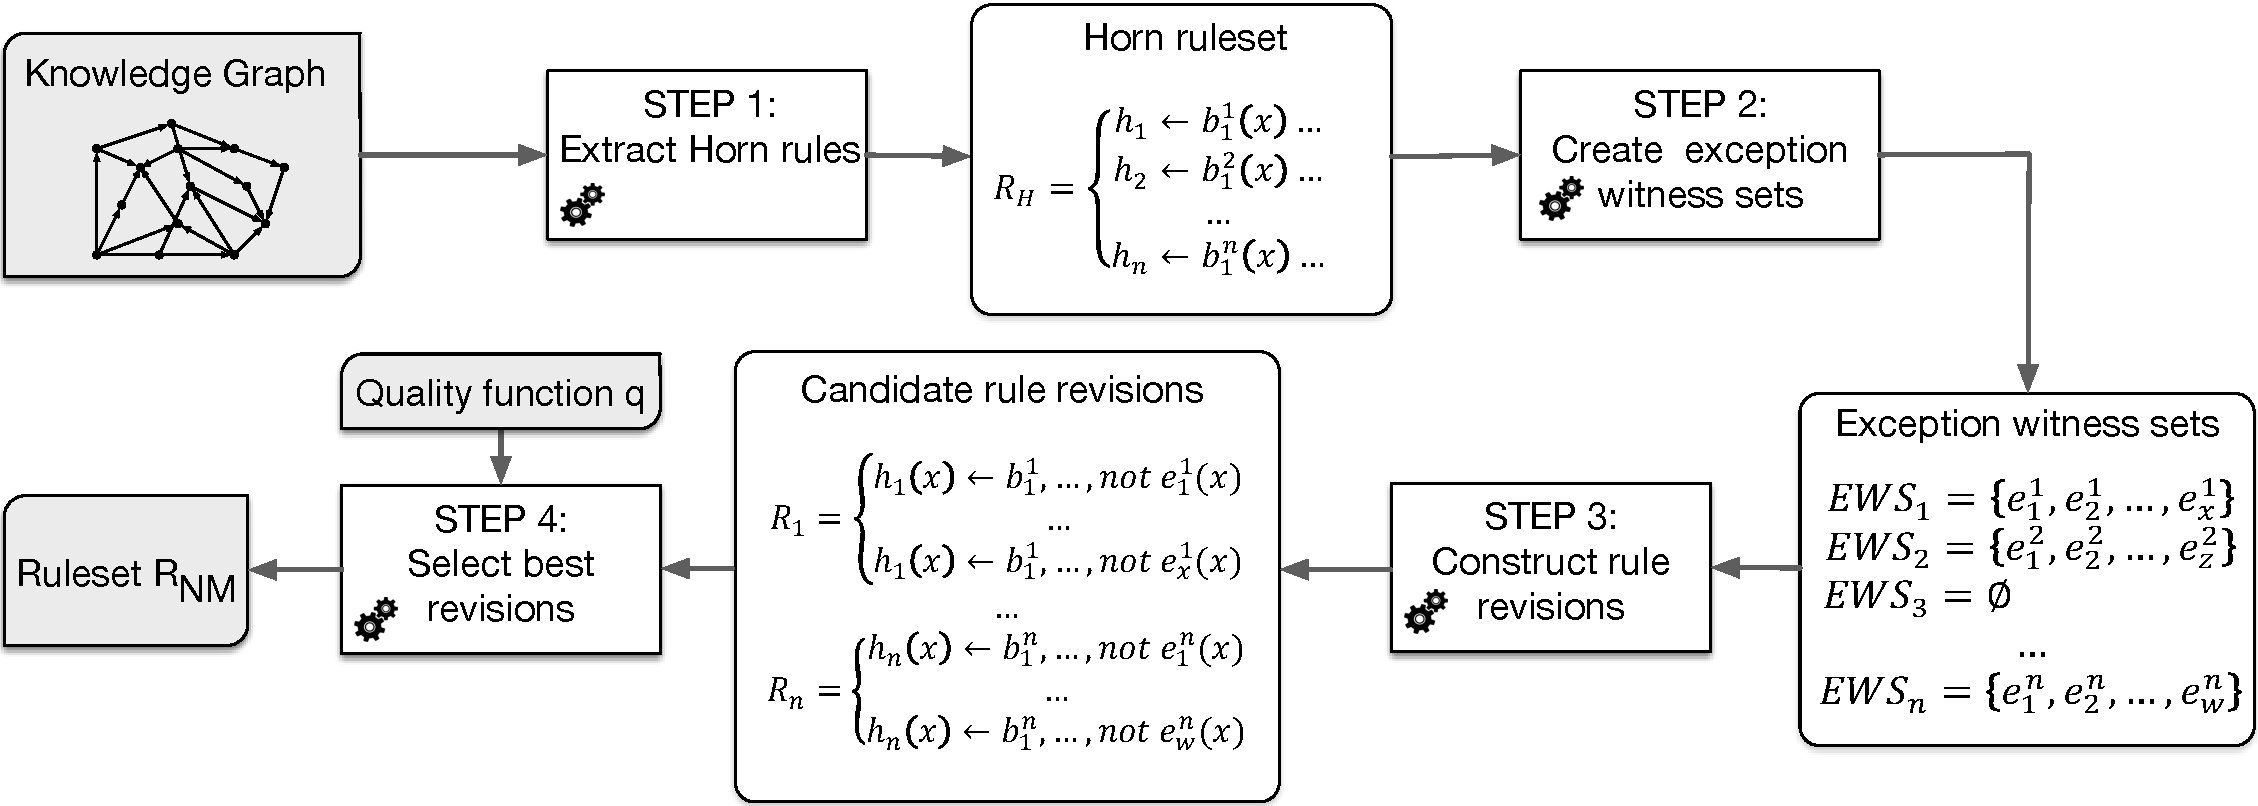
\includegraphics[width=\textwidth]{figures/overview}
\caption{Rule revision process by~\cite{gad2016,rumis}}
\label{fig:iswc_process}
\end{figure}
\leanparagraph{Program consistency maximization approaches} In both \cite{gad2016} and RUMIS~\cite{RUMIS} introduced an approach to revise a set of Horn rules $R_H$ learned from KGs into nonmonotonic set $R_{MN}$ by adding at most one negated atom to each rule. The final revision is chosen such that the average quality of the Horn rule set is maximized while the conflict between the predictions of the different rules are minimized. 

In order to estimate the conflict between the predictions of the rules, they introduce the notion of auxiliary rules, concretely, for a rule 
\[r:H \leftarrow B, \naf E\] an auxiliary version is \[r:\mi{not\_H} \leftarrow B, E\] where $\mi{not\_H}$ is a fresh predicate indicating that $H$ will not be derived by this rule. The number of grounded pairs $\tuple{H,\mi{not\_H}}$ in the answer set generated by the rule set and the KG indicates the degree of conflict.


Figure~\ref{fig:iswc_process} shows the rule revision steps as described by~\cite{gad2016} (and similarly RUMIS). 

First, Horn rules are extracted from the KG. In the case of~\cite{gad2016}, the KG is first projected from the binary relations into unary one by introducing new predicates that combines the original predicate and the class of the object part (aka propositionalization). For example, given facts $\mi{isMarriedTo(bob, alice)}$ and $\mi{researcher(alice)}$, the first can be projected into $\mi{isMarriedTo\_researcher(bob)}$. Using the class of the object instead of the instances allows learning patterns. A traditional item set mining approach to obtain the Horn rules $R_H$ from the projected KG. RUMIS takes as input a rule set learned by using any positive rule mining system such as ~\cite{amie,op,rdf2rules}.  

Second, in order to construct the exception witness set (EWS), for each rule $r$ the normal and abnormal  sets are defined: the normal set is the set of the substitutions of the variables $\mathcal{V}$ with the entities such that satisfy both the head and the body of the rule $r$, while the abnormal set contains the  substitutions for which the rule body is satisfied but not the head.

Formally, for each rule $r \in \cR_H$, let $\mathcal{V}$ be the set of variables of $r$, the normal and abnormal sets are respectively defined as follows:
\begin{itemize}
\item $NS(r, \cG) = \{\theta \mid head(r)\theta, body(r)\theta \subseteq \cG\}$
\item $ABS(r, \cG) = \{\theta \mid body(r)\theta \subseteq \cG , head(r)\theta \notin \cG\}$\\
where $\theta: \mathcal{V} \rightarrow \cC$.
\end{itemize}

\begin{example}
Consider the KG $\cG_1$ and $r_1$ as before, the normal set for $r_1$ is $NS(r_1,\cG_1)=\{\theta_1, \theta_2 ,\theta_3\}$, where $\theta_1 = \{X/brad, Y/ann, Z/berlin\}$,\\  $\theta_2 = \{X/john, Y/kate, Z/chicago\}$ and $\theta_3 = \{X/sue, Y/li, Z/beijing\}$.\\ and the abnormal set, $ABS(r_1,\cG_1)=\{\theta_4,\theta_5, \theta_6\}$, \\such that $\theta_4=\{X/bob, Y/alice, Z/berlin\}$,  $\theta_5=\{X/clara, Y/dave, Z/chicago\}$, and $\theta_6=\{X/mat, Y/lucy, Z/amsterdam\}$.
\qed
\end{example}

 \gad{stopped here! details to be added}
 
Second, based on the (ab)normal substitutions, let $\mathcal{X} \subseteq \mathcal{V}$, we compute the Exception Witness Set (EWS) for each $r \in \cR_H$, which is a maximal set of predicates $EWS(r,\cG,\mathcal{X}) = \{p_1,...,p_k\}$ s.t.:
\begin{itemize}
\item $\forall i \in \{1,..,k\} : \exists \theta \in ABS(r, \cG)\ s.t.\ p_i(\mathcal{X}\theta) \in \cG$, and 
\item $\forall \theta \in NS(r,\cG) :  p_1(\mathcal{X}\theta), ...,p_k(\mathcal{X}\theta) \notin \cG$
\end{itemize}



%
%\leanparagraph{RUMIS} RUMIS starts with a set of \textit{closed} Horn rules $\cR_H$, which can be learned by using any positive rules mining systems \cite{amie,op,rdf2rules}, and then finds the single best exception for each Horn rule $r \in \cR_H$ to obtain a revised set of nonmonotonic rules $\cR_{NM}$ such that the difference between $\cG^i$ and $\cG^i_{R_{NM}}$ is minimized. Below is the overview of how RUMIS revises the ruleset $\cR_H$ to achieve $\cR_{NM}$.
%\begin{enumerate}
%\item
% First, for each rule $r \in \cR_H$, let $\mathcal{V}$ be the set of variables of $r$, the normal substitutions and abnormal substitutions are respectively extracted as follows:
%\begin{itemize}
%\item $NS(r, \cG) = \{\theta \mid head(r)\theta, body(r)\theta \subseteq \cG\}$
%\item $ABS(r, \cG) = \{\theta \mid body(r)\theta \subseteq \cG , head(r)\theta \notin \cG\}$\\
%where $\theta: \mathcal{V} \rightarrow \cC$.
%\end{itemize}
%Informally, the normal and abnormal substitutions stand for the substitutions of variables $\mathcal{V}$ with the entities such that the rule $r$ holds (both the head and the body hold) and does not hold (only the body holds) in $\cG$, correspondingly.
%\begin{example}
%Consider the KG $\cG_1$ and $r_1$ as before, we have $NS(r_1,\cG_1)=\{\theta_1, \theta_2 ,\theta_3\}$, where $\theta_1 = \{X/brad, Y/ann, Z/berlin\}$, $\theta_2 = \{X/john, Y/kate, Z/chicago\}$ and $\theta_3 = \{X/sue, Y/li, Z/beijing\}$. Similarly, $ABS(r_1,\cG_1)=\{\{X/bob, Y/alice, Z/berlin\},$ $\{X/clara, Y/dave, Z/chicago\},$ $\{X/mat, Y/lucy, Z/amsterdam\}\}$.
%\qed
%\end{example}
%\item 
%Second, based on the (ab)normal substitutions, let $\mathcal{X} \subseteq \mathcal{V}$, we compute the Exception Witness Set (EWS) for each $r \in \cR_H$, which is a maximal set of predicates $EWS(r,\cG,\mathcal{X}) = \{p_1,...,p_k\}$ s.t.:
%\begin{itemize}
%\item $\forall i \in \{1,..,k\} : \exists \theta \in ABS(r, \cG)\ s.t.\ p_i(\mathcal{X}\theta) \in \cG$, and 
%\item $\forall \theta \in NS(r,\cG) :  p_1(\mathcal{X}\theta), ...,p_k(\mathcal{X}\theta) \notin \cG$
%\end{itemize}
Intuitively, $\mathcal{X}$ is set containing of either 1 or 2 variables of $\mathcal{V}$ corresponding to the usage of unary or binary exception. While the first condition ensures that the exception does affect the abnormal substitutions of the rule, the second condition ensures that it does not affect the rule's normal substitutions part. In other words, $EWS(r,\cG,\mathcal{X})$ contains all possible exceptions to be added to $r$ at variables of $\mathcal{X}$, such that the addition of the exception should result in the rule $r'$, satisfying $\textit{b-supp}(r', \cG) < \textit{b-supp}(r, \cG)$ and $\textit{r-supp}(r', \cG) = \textit{r-supp}(r, \cG)$. Intuitively, the application of exception should lead to the decrease of the body support, but not lead to the decrease of
the rule support, i.e., exceptions should explain the absence of predictions expected to be in the graph rather then their presence.
\begin{example}
We have $EWS(r_1,\cG_1,\{X\}) = \{artist\}$ and $EWS(r_1,\cG_1,\{Y\}) = \{researcher\}$.
\qed
\end{example}
Combining all possible exceptions at different variables of rule we have:
\[EWS(r,\cG) = \bigcup_{\forall\mathcal{X}\subseteq \mathcal{V}}EWS(r,\cG,\mathcal{X})\]

%\item 
For each rule $r \in \cR_H$, we now have $EWS(r,\cG)$ containing all of its exception candidates. The final step is to rank these exceptions based on some scoring function and select the one with the highest score to build the rule with exception $r'$ in $\cR_{NM}$. At this point, several exception scoring functions have been proposed by RUMIS \cite{rumis}.
%Let $r_i^j$ be the nonmonotonic rule built from $r_i \in \cR_H$ by adding $j$-th exception of $EWS(r_i,\cG)$, the introduced exception scoring functions are as follows:
\begin{itemize}
\item \textbf{Naive (N)}: is the simplest scoring function, which choosing the exception with the highest value of some standard rule measure $rm$. RUMIS system uses conviction as the rule measure $rm$.
\item \textbf{PM}: invoke the novel concept of \textit{partial materialization}. The idea behind it is to rank candidate exceptions not based on $\cG$ as in Naive, but rather on its
extension with predictions produced by other rules in $\cR_H$, thus ensuring a crosstalk between the rules.
\item \textbf{OPM}: stands for \textit{ordered partial materialization}. This exception scoring function is similar to \textbf{PM}, but also takes into account the order of rules in $\cR_{H}$, which is defined based on some rule measure (e.g. \textit{r-supp} in RUMIS).

\thi {Should I describe the 3 ranking measures in more detail?}
\end{itemize}
%\end{enumerate}





%\leanparagraph{Learning rules with external resources}
\section{Discussion and Outlook}\label{sec:disc}

\begin{figure}[t]
\centering
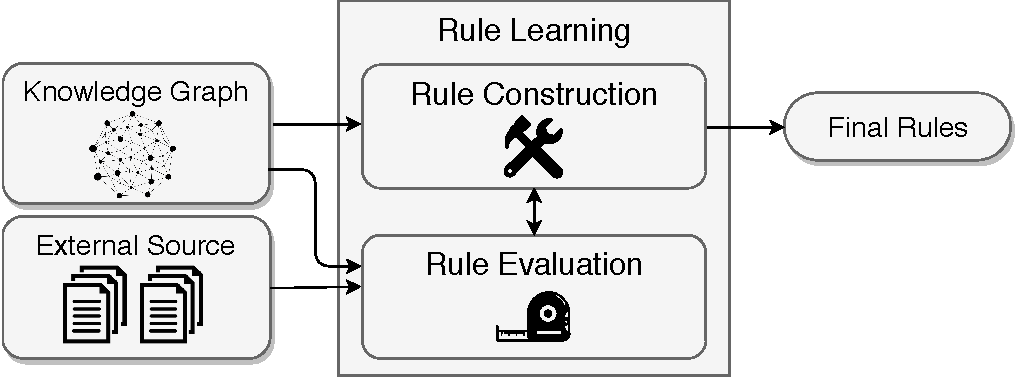
\includegraphics[width=8cm]{figures/discussion_overview}
\caption{Rule learning with external sources}
\label{fig:discussion_overview}
\end{figure}

In this tutorial, we have presented a brief overview of the current techniques on rule induction from knowledge graphs and have demonstrated how reasoning over KGs using the learned rules  can be exploited for KG completion. % discussed the different approaches for rule induction and reasoning over real-life KGs. We briefly illustrated the common method for KG construction and the incompleteness and inaccuracy challenges they face. We also illustrated the difference between \textit{Horn} and  \textit{nonmonotonic} logic program and their connection to association rules. Later, we reviewed some of the existing systems for constructing Horn rules from KGs and the proposed rule evaluation measurements under OWA. Furthermore, we discussed the exiting inductive and abductive methods for learning nonmonotonic rules and their applicability over real-life KGs. Finally, we discussed rule revision approach RUMIS, which tries to capture exceptional cases to achieve accurate and consistent predictions. 

While the problem of rule-based KG completion has recently gained an increasing attention, several interesting research directions are still left unexplored. % Despite the advances in rule learning, the existing methods still learn limited formats for rules, \eg closed rules, with even restrictive language bias.
% Additionally, they are still prone to KG incompleteness and not being able to determine the possible gaps in the data under OWA. These challenges lead to the generation of uninteresting and noisy rules. Follows some possible directions to overcome such challenges. 


\leanparagraph{Learning rules over probabilistic data} KG automatic and semi-automatic construction leads to inaccurate instances. Nevertheless, existing rule learning approaches over KG model the KG as set of certain triples; leading to less accurate rules, and hence, predictions. Modeling the KG as uncertain data source and learn rules over weighted triples should reduce the effect of inaccurate facts in the KG Addressing the rule learning over weighted data has been studied under probabilistic ILP%, where given a set of probabilistic examples for grounded atoms and a target predicate $H$, the task is to learn rules for predicting probabilities of atoms for $H$
~\cite{probfoil,DBLP:conf/ijcai/RaedtDTBV15,DBLP:conf/clima/CorapiSIR11}.  
However, applying these techniques to our setting requires a full materialization of the probability function,
which quickly grows to sizes that ILP methods cannot handle. Adapting probabilistic rule learning approaches has not yet been studied well under the scale of real-life KGs.


\leanparagraph{Rule learning with external sources} 
One promising direction is to consider pieces of evidence from other external resources while extracting the rules from KGs and estimating their quality 
(see Figure~\ref{fig:discussion_overview}). This external resource can be of a different nature ranginf from %either be 
a human expert giving feedback about the correctness of a given rule as done in~\cite{Dzyuba2017} in the context of frequent itemset mining, or a dedicated fact-checking engine that given a fact, e.g., $\mi{bornIn(einstein,ulm)}$ relies on the existing Web resources for estimating its truthfulness. This amounts to utilizing such automated fact-checking systems as Defacto~\cite{defacto} or FactChecker~\cite{factchecker} in the rule induction process. 

An alternative relational learning method for KG completion is to learn representations (i.e. embeddings) of entities and relations from a given KG possibly enriched with additional information sources (e.g., text) with the % propose
purpose of estimating the likelihood of unseen facts (see \cite{Wang2017} for overview). However, the
predictions produced by such approaches are not interpretable~\cite{Shakerin2018}. Interlinking these statistical methods with inductive rule learning is a promising further direction.

\leanparagraph{Neural-based rule learning} Utilizing embedding models for rule learning is a new research direction that has recently gained attention \cite{DBLP:conf/nips/YangYC17,DBLP:journals/corr/YangYHGD14a}. Existing methods are purely statistics-based, i.e., they reduce the rule learning problem to algebraic operations on neural-embedding-based representations of a given KG.  \cite{DBLP:journals/corr/YangYHGD14a} constructs rules by modeling relation composition as multiplication or addition of two relation embeddings. The authors of \cite{DBLP:conf/nips/YangYC17} propose a differentiable system for learning models defined by sets of first-order rules that exploits a connection between inference and sparse matrix multiplication \cite{DBLP:journals/corr/Cohen16b}. However, existing approaches pose strong restrictions on target rule patterns, which often prohibit learning interesting rules, e.g. non-chain-like or exception-aware ones.

\leanparagraph{Learning other rule forms}
%Prominent rule learning approaches only extract normal $closed$ logical rules, which may not capture all interesting patterns. However, 
Inducing rules of  advanced forms, e.g., %other rule forms such as 
rules with disjunction (\eg $hasBrother(X,Y) \vee hasSister(X,Y) \leftarrow hasSibling(X,Y)$, or $livesIn(X, North Korean) \vee livesIn(South Korean) \leftarrow speaks(X, Korean) $), or rules with existential quantifiers in the head (\eg $\exists Y: playsInstrument(X, Y) \leftarrow$ $musician(X),bandMember(X,Z)$) is an interesting topic to study. Several recent works on mining keys in KGs \cite{vickey,DBLP:conf/www/LajusS18} and detecting mandatory relations are relevant, but they do not directly address the mentioned rule forms. A combination of techniques from relational rule learning \cite{DBLP:books/daglib/0021868} and propositionalization approaches \cite{propos} can be made use of, yet it is unclear how to detect KG parts that are worth propositionalizing; the details are to be explored. % can encode more interesting patterns
% Even though these
While rules with existential variables in the head may not directly infer new facts, they may reflect surprising patterns in the data and, moreover,  can be used as a guidance for the information retrieval approaches.

Rules that reflect correlations between edge counts in KGs such as \emph{``If you have two siblings then you parents are likely to have 3 children''} have been studied in \cite{carl}. Inducing more general rules, reflecting mathematical functions one edge counts is still an open problem, which due to the large search space of possible hypothesis is far from trivial.

% \leanparagraph{Learning temporal rules} 
% Current approaches extract the rules from the directly stated entities and relations. More promising direction would be to learn patterns over more unstated relations such as temporal rules. For examples, KGs usually contain the dates of the events, \eg $\mi{dateOfbirth}$ or $happenedOn$ which is sparse data and requires arithmetic operator to make use of them, \eg $before(X,Y)$, $after(X,Y)$. Learning interesting rules over this data is still not well studied.
Learning temporal rules and constraints such as \emph{``You cannot graduate from a university before being born''} is another promissing future work direction. Deductive reasoning over temporal KGs has been recently considered in \cite{DBLP:conf/aaai/ChekolPSS17}; however the inductive setting has not yet been studied in full details to the best of our knowledge.

\leanparagraph{Hybrid rule learning techniques} Inducing rules from text by exploiting natural language processing (NLP) techniques has been studied in several works \ds{Insert citations}. Combining these linguistics-based methods with inductive rule learning from KGs has a great potential. Indeed, the number of predicates in most encyclopedic KGs is rather limited, since they are primarily extracted from Wikipedia; this prohibits the extraction of many interesting rule patterns such as ``\ds{TODO: insert. The previous rule about injured people has a negative flavor for being in the end of the article and it needs more motivation}''. %, like % where such non-standard facts as ``Einstein worked with Feynmen'' are rarely added. The number of predicates is limited in most of the KGs. Therefore, sometimes it is hard to learn interesting patterns from the KG only. In contrast, textual resources are rich with verbal phrases that indicate events or relations. However, learning the simplest rules from unstructured resources is challenging. Therefore, it worth investigating constructing hybrid rules that combine both resources.  For example, to learn a rule such as

% \begin{align*}
% \mi{participatedIn(X,Y)} \leftarrow & \mi{playsFor(X,Z)}, \mi{competes(Z,Y)},\\ & \naf injuredDuring(X,Y)
% \end{align*}
% \ds{would suggest to add a different rule here, this }
% The rule encodes that a player participates in a championship if he plays for a competing team unless he was injured during the championship. Learning the positive part of the rule can be easily done over the KG, yet the last one is more common to find in the text. 




%\section{Discussion and Outlook}
%\label{sec:discussion_outlook}
%Toward the rule-based KG completion problem, a number of future directions could be put into consideration.
%\subsubsection{Rule Learning with External Source.}

%In most of rule learning systems have been proposed \cite{amie,op,rdf2rules}, while their rule construction methods may vary, the core of them is at the proposed rule evaluation metric. Various rule measures have been introduced, from the simplest to the most sophisticated one. Nevertheless, most of them are computed based on only the given graph, and cover only a small subset of local patterns in the KG, thus might wrongly estimate the quality of extracted rules since real-world KGs are usually highly incomplete.
%
%One promising possibility to tackle this problem is to incorporate external related data from outside of the KG. The overview of such rule learning system could be described in Figure \ref{fig:discussion_overview}. The KG related external data can be extracted from many sources (e.g. crowd-sourcing, Web-extraction), and is obviously useful not only for rule evaluation, but also for rule construction over the KG. For instance, external data can give some feedback about the quality of predicted facts in several forms such as binary decision (\ie true or false) or a likelihood score. This feedback could be then taken into account for rule quality evaluation or exception capturing. In addition, external KG meta-data could gives some information about the existence of certain types of facts within the KG (as exploited in CARL~\cite{carl}). Moreover, we can also somehow learn rules directly from the text and then apply them back to the KG.
%
%An alternative relational learning method for KG completion is to learn representations (i.e. embeddings) of entities and relations for predicting likelihood of unseen facts. While these methods capture global patterns in the data, the predictions that they produce are not interpretable~\cite{Shakerin2018}. Many such models are been proposed \cite{Wang2017}, in which some of them could even be extended with additional unstructured knowledge (e.g., text corpus). Hence, integrating these embedding models into the rule learning approach might be a potential solution for the problem of rule-based KG completion.
%\subsubsection{Learning Various Rule Forms}
%In the KG completion problem, as mentioned, most of the rule mining approaches only mine $closed$ rules. Nevertheless, other form of rules might be also interesting. For example, rules with disjunction (e.g. $isMale(X) \vee isFemale(X) \leftarrow isPerson(X)$), rules with quantifier (e.g. $(\exists Y: playsInstrument(X, Y)) \leftarrow isMusician(X))$). Even though these kinds of rule do not directly make predictions on the knowledge graph since we do not know exactly which facts of the head are true, they might give us some useful constraints about the knowledge graph.

%\section{Conclusion}




% ---- Bibliography ----
%
% BibTeX users should specify bibliography style 'splncs04'.
% References will then be sorted and formatted in the correct style.
%
 \bibliographystyle{splncs04}
 \bibliography{references}
%

\end{document}
